\documentclass{article}
\usepackage[utf8]{inputenc}
\usepackage[english]{babel}
\setlength{\oddsidemargin}{0.25 in}
\setlength{\evensidemargin}{-0.25 in}
\setlength{\topmargin}{-0.6 in}
\setlength{\textwidth}{6.5 in}
\setlength{\textheight}{8.5 in}
\setlength{\headsep}{0.75 in}
\setlength{\parindent}{0 in}
\setlength{\parskip}{0.1 in}
\usepackage{xspace}
\usepackage{comment}
\usepackage{amssymb, amsmath, amsfonts, amsthm, graphics, mathrsfs, enumitem, tikz-cd}
\usepackage[hmargin=1 in, vmargin = 1 in]{geometry}
\usepackage{changepage}
\usepackage{array}

\usepackage{nameref}
\usepackage{caption}
\usepackage{graphicx}
\usepackage{natbib}
\usepackage[bookmarksopen,
bookmarksdepth=2,
breaklinks=true,
colorlinks=true,
urlcolor=blue,
citecolor=blue]{hyperref}

\usepackage{float}

% change outlook of empty set
\let\emptyset\varnothing

\newtheorem{theorem}{Theorem}[section]
\newtheorem{corollary}{Corollary}[theorem]
\newtheorem{lemma}[theorem]{Lemma}
\newtheorem{claim}{Claim}[section]
\theoremstyle{definition}
\newtheorem{definition}{Definition}[section]

\newcommand{\nghd}{neighborhood\xspace}
\newcommand{\fgrp}{$\pi_{1}$}
\newcommand{\topspace}[1]{$(#1, \tau_{#1})$}

%Blackboard bold letters.
\renewcommand{\AA}{\mathbb{A}}
\newcommand{\BB}{\mathbb{B}}
\newcommand{\CC}{\mathbb{C}}
\newcommand{\DD}{\mathbb{D}}
\newcommand{\EE}{\mathbb{E}}
\newcommand{\FF}{\mathbb{F}}
\newcommand{\GG}{\mathbb{G}}
\newcommand{\HH}{\mathbb{H}}
\newcommand{\II}{\mathbb{I}}
\newcommand{\JJ}{\mathbb{J}}
\newcommand{\KK}{\mathbb{K}}
\newcommand{\LL}{\mathbb{L}}
\newcommand{\MM}{\mathbb{M}}
\newcommand{\NN}{\mathbb{N}}
\newcommand{\OO}{\mathbb{O}}
\newcommand{\PP}{\mathbb{P}}
\newcommand{\QQ}{\mathbb{Q}}
\newcommand{\RR}{\mathbb{R}}
\renewcommand{\SS}{\mathbb{S}}
\newcommand{\TT}{\mathbb{T}}
\newcommand{\UU}{\mathbb{U}}
\newcommand{\VV}{\mathbb{V}}
\newcommand{\WW}{\mathbb{W}}
\newcommand{\XX}{\mathbb{X}}
\newcommand{\YY}{\mathbb{Y}}
\newcommand{\ZZ}{\mathbb{Z}}

\newcommand{\Z}{\mathbb{Z}}
\newcommand{\N}{\mathbb{N}}
\newcommand{\Q}{\mathbb{Q}}
\newcommand{\R}{\mathbb{R}}
\newcommand{\C}{\mathbb{C}}
\newcommand{\Bil}{\text{Bil}}
\newcommand{\Ob}{\text{Ob}}

\newcommand{\isom}{\cong} %The isomorphism symbol
\newcommand{\union}{\cup}
\newcommand{\intersection}{\cap}
\newcommand{\bigunion}{\bigcup}
\newcommand{\bigintersection}{\bigcap}
\newcommand{\disjointunion}{\sqcup}
\newcommand{\bigdisjointunion}{\bigsqcup}

% use macro to allow new word to stand out
\newcommand{\newword}[1]{\textbf{\emph{#1}}}

\newcommand{\mainpoint}[1]{
\noindent
\framebox{\parbox{\textwidth}{{\textbf{Main point:} #1}}}
}

% replace clear qed with filled black square
% \renewcommand\qedsymbol{$\blacksquare$}

% the following rules allow the numbering schemes to work with regards to each meeting number
\newcounter{lecnum}
\renewcommand{\thepage}{\thelecnum-\arabic{page}}
\renewcommand{\thesection}{\thelecnum.\arabic{section}}
\renewcommand{\theequation}{\thelecnum.\arabic{equation}}
\renewcommand{\thefigure}{\thelecnum.\arabic{figure}}
\renewcommand{\thetable}{\thelecnum.\arabic{table}}

% sets the heading
\newcommand{\lecture}[4]{
   \pagestyle{myheadings}
   \thispagestyle{plain}
   \newpage
   \setcounter{lecnum}{#1}
   \setcounter{page}{1}
   \noindent
   \begin{center}
   \framebox{
      \vbox{\vspace{2mm}
    \hbox to 6.28in { {\bf \small Uniformization Theorem, Flat Connections and Belyi Maps
	\hfill Summer 2019} }
       \vspace{4mm}
       \hbox to 6.28in { {\Large \hfill Meeting #1: #2  \hfill} }
       \vspace{2mm}
       \hbox to 6.28in { {\it Date: #3 \hfill Scribe: #4} }
      \vspace{2mm}}
   }
   \end{center}
   \markboth{Meeting #1: #2}{Meeting #1: #2}
}

% for definitions
\newenvironment{keyterm}[1]{ 
    \begin{definition}{\emph{#1}}\end{definition}
    \vspace{-2ex}
}

% for boxed terms
\newenvironment{boxed_q}
    {\begin{flushleft}
    \begin{tabular}{|p{0.9\textwidth}|}
    \hline\\
    }
    { 
    \\\\\hline
    \end{tabular} 
    \end{flushleft}
}

\title{
    Math REU 2019: Uniformization Theorem, Belyi Maps and Fuchsian Ordinary Differential Equations
}
\author{
    Drimik Roy\\
    Zachary Halberstam\\
    Dr. Caleb Ashley
}
\date{Summer 2019}

\begin{document}
\maketitle

\section{Notes for the reader}
These notes were created for my understanding of certain concepts during my Math REU at the University of Michigan. The final REU paper that I (Drimik) presented references the notes here in case the paper was unable to investigate a topic fully. There may be aspects of the notes that are left incomplete; most notes are cited from their original sources so that the reader may visit them for a more in-depth explanation. Please do email \href{mailto:drimikr@umich.edu}{drimikr@umich.edu} if any facts, theorems etc. are incorrectly stated! Thank you.

\section{Goals}
\label{sec:goals}
There will be an emphasis on understanding these statements and several proofs of the Uniformization theorem with being able to construct manifolds (surfaces) and to \textbf{develop the tools to tell manifolds apart}.

Towards the end, there will be discussion of \newword{Dessin d'enfants}, which are graph embeddings on Riemann surfaces.

The first few meetings will emphasize on the construction of the Riemann surfaces. A robust manner to do so is through \emph{quotient construction}. The Uniformization theorem serves as a way to construct Riemann surfaces. Investigation of Dessins to the Riemann-Hilbert problem is presented and of exploring how solution to Fuchsian ODE's can be translated into the language of combinatorial objects.

\lecture{1}{Introduction and Definitions}{May 7th}{Drimik Roy}
\setcounter{section}{0}
We will be introducing several terms and definitions as a background of understanding. Introductory notes regarding Riemannian spheres, Complex planes and hyperbolic planes are recorded in \textit{Notability} for the Bonahon Chapters 1 through 3 \cite{bonahonlow}.

\section{General Key Terms}
\begin{keyterm}{Riemann Surface} 
A one dimensional complex manifold; that is, 2nd countable, Hausdorff space $\Sigma$ such that $\forall p \in \Sigma$, $\exists$ \nghd $U_{p}$ and homemorphism $\phi_{p}: U_{p} \to V_{p} \subseteq \CC$ satisfying the following compatibility properties: if for $p,q \in \Sigma$ we have that $U_{p} \intersection U_{q} \ne \emptyset$, then the \newword{transition function} of $\phi_{p} \circ \phi_{q}^{-1}$ is \newword{holomorphic}.

Note that we usually identify the \nghd and homeomorphism with the pair $(U_{p}, \phi_{p})$ where the former term is known as the \newword{coordinate} or \newword{affine patch} and the latter is the \newword{coordinate chart}.  
\end{keyterm}

\begin{keyterm}{Uniformization Theorem}
A simply connected (for more on connectedness, look at \nameref{sec:m2_connectedness} in Section \ref{sec:m2_connectedness}) Riemann surface is biholomorphic to precisely one of the following \cite{uniformization_northwestern}:
\begin{itemize}
    \item the unit open disk $\DD$
    \item the complex plane $\CC$
    \item the Riemann Sphere $\hat{\CC}$
\end{itemize}
\end{keyterm} 

\begin{keyterm}{Hausdorff space}
A topological space in which for any two distinct points, there exists a neighborhood of each that is disjoint from the neighborhood of the other.
\end{keyterm}

\begin{keyterm}{Second countable}
A topological space $(X,\tau)$ is said to be \newword{second countable} if there exists a basis $\BB$ of $\tau$ that is countable. An equivalent definition would be is that for an arbitrary $x \in X$ and any $U_{x}$ as an open neighborhood, $U_{x}$ admits a countable local base.
\end{keyterm}

\subsection{Function types}

\begin{keyterm}{Homeomorphisms}
A continuous function between \textit{topological spaces} that has a continuous inverse function.
\end{keyterm}

\begin{keyterm}{Holomorphisms}
A \textit{complex-valued} function that is complex-differentiable at every point in its domain for some \nghd of the point.

\textit{Biholomorphisms} are holomorphisms that have an inverse that is also holomorphic.
\end{keyterm}

\begin{keyterm}{Diffeomorphisms}
A smooth, invertible, and differentiable function on manifolds i.e. an \textit{isomorphism on smooth manifolds}.
\end{keyterm}

Note that these terms are defined more in relation with Category Theory in Section \ref{sec:m1_category_theory}.

\section{Exploration of the complex projective line $\CC\PP^{1}$}
We define 

\begin{align}
\begin{split}
    \CC\PP^{1}
    &= \{\text{lines through the origin in } \CC^{2}\}\\
    &= \CC^{2}\text{\textbackslash}\{0\}/\sim
    \label{eqn:m1_cp1}
\end{split}
\end{align}

This set defined is a subset of $\CC^{2}$ of all pairs $(\alpha, \beta)$ where modulo the equivalence relation we have $(\alpha, \beta) \sim (\lambda\alpha, \lambda\beta)$ for all \textit{nonzero} complex numbers $\lambda$. In other words, $\CC\PP^{1}$ is the projective space of all lines through the origin in $\CC^{2}$.

The reason we disallow $\lambda$ as assuming the zero complex number is because all the complex pairs of $\CC^{2}$ which would be equivalent to the origin under $\sim$, and thus, every element of $\CC^{2}$ would belong to the same equivalence class. Similarly, we the pair $(0,0) \in \CC^{2}$ is excluded as well from this study.

\mainpoint{$\CC\PP^{1}$ is the set of all 1-dimensional subspaces of $\CC^{2}$.}

\subsection{Stereographic projection}
In geometry, the \newword{Stereographic Projection} is a function (mapping) $\phi$ that projects a sphere onto a plane. How this function is constructed is in relation to a \newword{projection point}, which is determined below as the north pole in Figure \ref{img:m1_steoregraphic_projection}. Note that every point $p$ on the sphere except at the projection point is uniquely identified with a point $p'$ on the Complex plane $\CC$ by extending the line between the projection point and $p$ onto the plane which is the mapping presented by $\phi$.

Wherever $\phi$ is defined, it is smooth and bijective and therefore a continuous map may be constructed between the topological spaces of the sphere and the plane. Since $\phi$ is bijective, the inverse map $\phi^{-1}$ is well defined and because $\phi$ is an open map (i.e. takes open sets to open sets), $\phi^{-1}$ is continuous. Hence, the function $\phi$ is a homemorphism between the sphere disregarding the projection point and the complex plane. 

\begin{figure}[H]
\centering
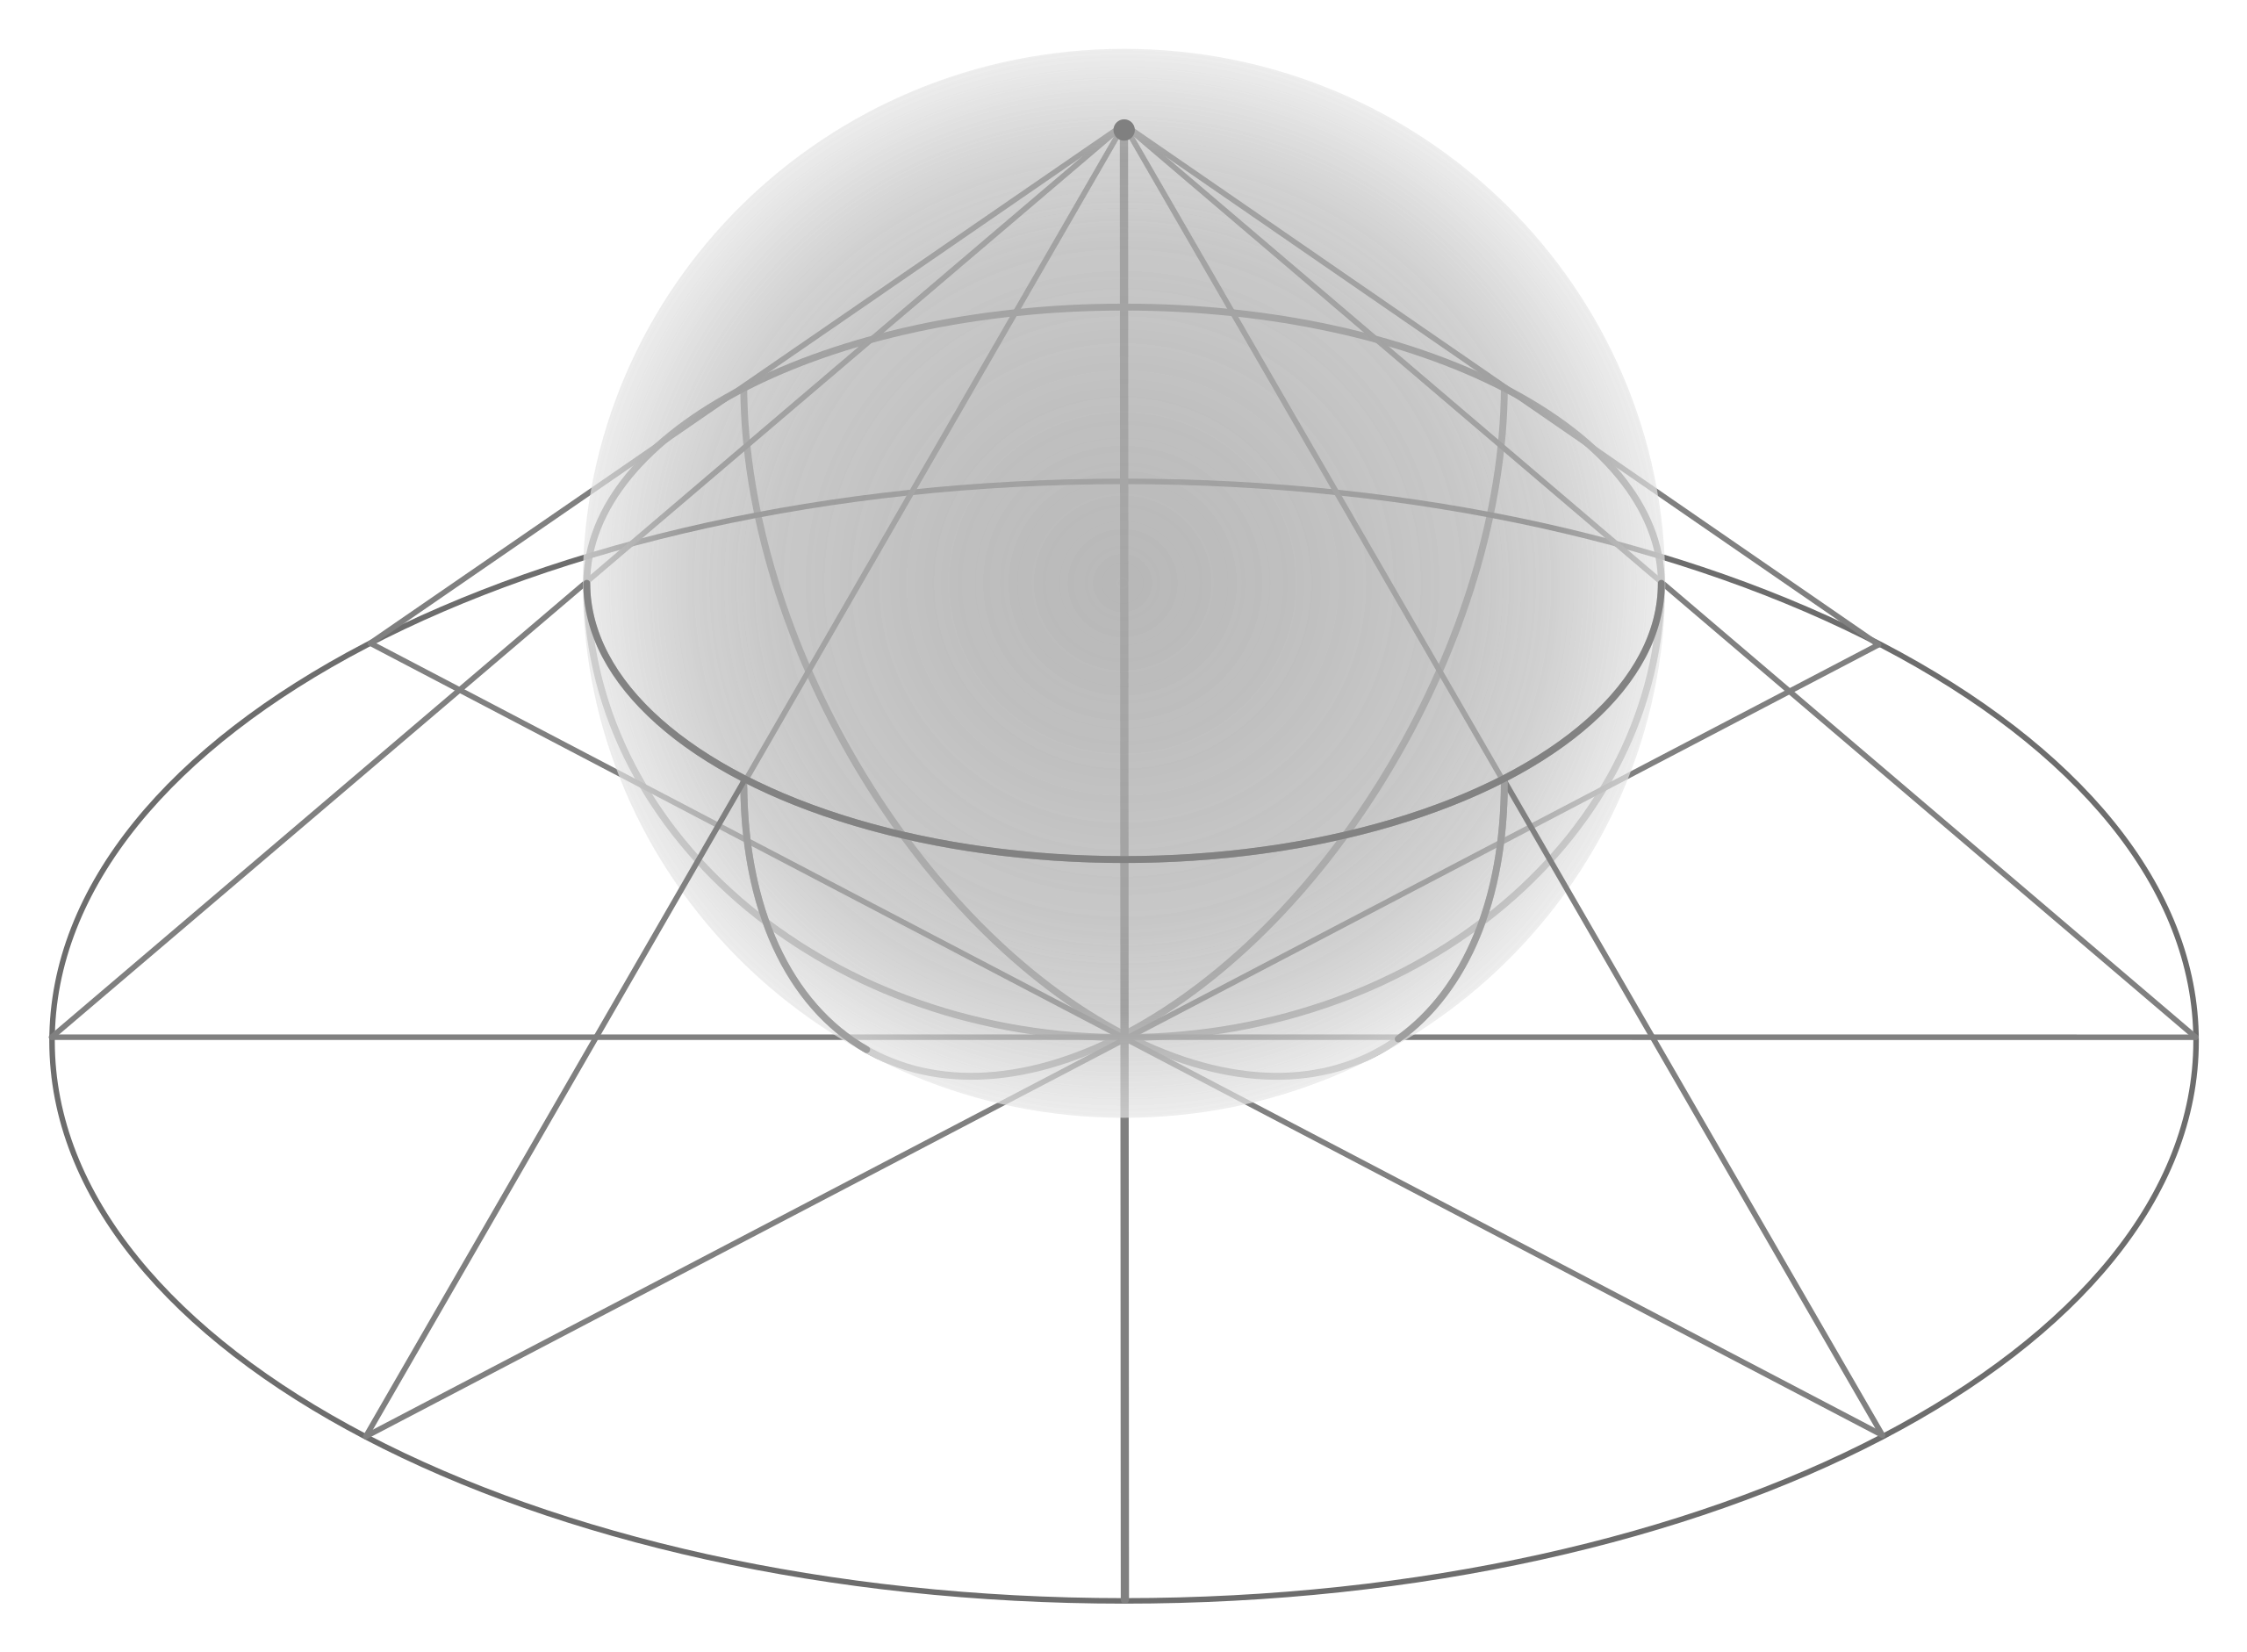
\includegraphics[width=10cm]{images/m1_stereographic_projection.png}
\caption{\small{Stereographic projection of $\SS^{2}$ to $\CC$} by disregarding the projection point of the north pole (image from \href{https://en.wikipedia.org/wiki/Stereographic_projection}{wikipedia})}
\label{img:m1_steoregraphic_projection}
\end{figure}

More generally, we have that the Stereographic projection can be applied to the n-sphere $\SS^{n}$ and be embedded into the (n+1)-dimensional Euclidean space $\EE^{n+1}$ if in fact the north pole is considered in the projection.

\mainpoint{There exists a homeomorphism from a sphere with a hole and a plane i.e. a sphere without a point is contractible into a plane.}

\subsection{Identification of $\CC\PP^{1}$ to $\hat{\CC}$}
Now, it has been established on the canonical mapping between a sphere $\SS^{2}$ without a point and the Complex plane $\CC$. We will now state why in fact the Riemannian sphere can be defined as exactly the complex projective line. In order to understand in depth the relationship between $\hat{\CC}$ and $\CC\PP^{1}$, some preliminary knowledge of quotient spaces will be stated, which will establish the projection mapping $\pi: X \to X/\sim$.

\subsubsection{Quotient spaces}
Let \topspace{X} be a topological space and $\sim$ be an equivalence relation defined on $X$. The \newword{quotient space} $Y=X/\sim$ is the set of equivalence classes of X i.e. $Y = \{[x] : x \in X\}$. What is critical is the \newword{quotient topology} of $Y$. The open sets of $Y$ are defined to the open preimage sets of the canonical projection map $\pi$ that maps each element to its equivalence class. In other words, 
$\tau_{Y} = \{U \subseteq Y : \pi^{-1}(U) \in \tau_{X}\} $.

By the definition of $\CC\PP^{1}$ in Equation \ref{eqn:m1_cp1}, the surjective map
\begin{align*}
    \pi: \CC^{2}/\{0\} &\to \CC\PP^{1}\\
    (z_{1}, z_{2}) &\mapsto [z_{1}:z_{2}]
\end{align*}

is the canonical projection map specified for our exploration. 

\begin{theorem}
The Riemann Sphere $\hat{\CC}$ can be defined as the complex projective line $\CC\PP^{1}$.
\end{theorem}

\begin{proof}
We will rely on the steoreographic projection defined in Section \ref{img:m1_steoregraphic_projection}, the homeomorphism associated $\phi$ and the use of the canonical projection mapping $\pi$ utilized to determine the quotient topology of $\CC\PP^{1}$ of the set $\CC^{2}/\{0\}$.

\underline{Case 1}: $z_{1} \ne 0$\\
Since the equivalence relation $\sim$ is defined as $(\alpha, \beta) \sim (\lambda\alpha, \lambda\beta)$ for all nonzero complex numbers $\lambda$, it follows that $[z_{1}:z_{2}] \sim [1:z]$ where $z = z_{2}/z_{1} \in \CC$. Note that in general, any arbitrary $z \in \CC$ can be constructed in such a way. Through the stereographic projection and the mapping $\phi$ as the homeomorphism, $\phi^{-1}$ allows the unique identification of any element from $z$ to $\hat{\CC}$ except at the north pole.

\underline{Case 2}: $z_{1} = 0$\\
In this scenario, $[z_{1}:z_{2}] \sim [0:1]$ by allowing $\lambda = z_{2}$. Fix this unique class $[0:1] \in \CC\PP^{1}$ as the north pole of $\hat{\CC}$. 

By Cases 1 and 2, the Riemann sphere can indeed be defined as the complex projective line.
\end{proof}

\section{Examples of Riemann Surfaces and Why}
\begin{enumerate}
    \item \textbf{Complex Plane} $\CC$ with coordinate patch $\CC$ itself (as $\CC$ is open in its own space with regards to $\tau_{E}$) with the homeomorphism $\phi: \CC \to \CC$ represented by the identity. Note the transition function between this patch and itself is just the identity, which is holomorphic. It follows that $\CC$ is a Riemann surface.
    \item \textbf{Riemann Sphere} $\hat{\CC}$ with two ordered pairs $(U_{j}, \phi_{j})_{j\in j}$ with $J=\{0, \infty\}$, claiming the ordered pairs construct an atlas of $\hat{\CC}$.
    \begin{itemize}
        \item $U_{0} = \CC$ with homeomorphism $\phi_{0}$ as the identify map.
        \item $U_{\infty} = \CC\text{\textbackslash}\{0\} \union \{\infty\}$ and $\phi_{\infty}$ with homeomorphism $\phi_{\infty}$ on $U_{\infty}$ as $\phi_{\infty}(z)=1/z \in \CC$. The map identifies $\infty$ to $0$.
    \end{itemize}
    
    Thus, $(U_{j}, \phi_{j})_{j\in j}$ indeed represents an atlas of the Riemann sphere and that the composition of these functions between the two distinct patches is $1/z$, which is holomorphic. Hence, we have a 1 dimensional complex manifold $\therefore \hat{\CC}$ is a Riemann surface.
        
\end{enumerate}

\section{Exploration of Category Theory}
\label{sec:m1_category_theory}
Categorically, there are three spaces we will explore and particular set of functions on each of these structures:
\begin{itemize}
    \item Topological spaces with homeomorphisms
    \item Smooth spaces with diffeomorphisms
    \item Complex spaces with biholomorphisms
\end{itemize}
        
\section{Questions}
\begin{enumerate}
    \item Clarification on 2nd countable, 1st countable, local base
    \item Understanding the relationship (anti)linear fractional maps $\phi:\hat{\C} \to \hat{\C}$ sending a circle of $\hat{\C}$ to a circle of $\hat{\C}$.
    \item Affine spaces
    \item IMPORTANT: transition maps $f(z) = 1/z$
\end{enumerate}

% MEETING 2
\lecture{2}{Homotopies, Isotopies, and Fundamental Groups}{May 8th}{Drimik Roy}
\setcounter{section}{0}
\section{Overview}
To understand the discussion of these algebraic topological concepts, the construction of Riemann surfaces through \newword{quotient construction} is defined as the construction defined by an action of the fundamental group acting by isometrics on a universal covering space. 

The notion of the fundamental group will require the understanding of what \newword{homotopies} are. Every Riemann surface can be explained as the quotient of one of the 3 simply connected Riemann surfaces - open disk, complex plane, Riemann sphere - by some group of isometries as the group of isometries is isomorphic to the fundamental group of the surface. These notions will be explored in the following meetings and claims will be proven.

This meeting mainly focused on definitions and concepts associated with homotopy theory, categories, and fundamental groups, which will be utilized heavily in the construction of Riemann surfaces as mentioned for following meetings.

Revision of important points:
\begin{enumerate}
    \item Manifolds are in our case both 2nd-countable and Hausdorff spaces with transition maps defined to compare charts between atlases. What is changing is the type of function the transition map is (e.g. if holomorphic, then we have a complex manifold or if smooth, then we have a smooth manifold).
    
\end{enumerate}

\section{General Key Terms}
\begin{keyterm}{Atlas}
An \newword{atlas} for a topological space $X$ is a collection $(U_{i}, \phi_{i})_{i \in I}$, where $I$ is an indexing set, of charts on $X$ such that $\bigunion_{i \in I} U_{i} = X$. 
\end{keyterm}

\section{Notions of Connectedness}
\label{sec:m2_connectedness}
Recall that a connected space is a topological space that cannot be written as the union of two disjoint nonempty open subsets. 

Let \topspace{X} be a topological space. A \newword{path} from $x$ to $y$ in a $X$ is a continuous function $f$ on the unit interval $[0,1]$ to $X$ where $f(0)=x$ and $f(1)=y$.

\begin{keyterm}{Path connected} 
$X$ is \newword{path connected} if there is a path $f$ for any two points in $X$.
\end{keyterm}

\begin{keyterm}{Simply connected}
$X$ is \newword{simply connected} if it is path connected and every loop in $X$ can be contracted into a point. 

Equivalently, $X$ is simply connected if is path connected and for any two paths $p,q$ of $X$ has the same start and endpoint (i.e. $p(0)=q(0)$ and $p(1)=q(1)$) and that $p$ can be continuously deformed into $q$ (explicitly, there is a homotopy between $p$ and $q$).
\end{keyterm}

\begin{theorem}
A path-connected topological space is connected.
\end{theorem}
\begin{proof}
Let \topspace{X} be a topological space. Suppose $X$ is disconnected. That is, $X = A \union B$ where $A,B$ are nonempty, disjoint, open subsets of $X$. Fix $x \in A, y \in B$. Since $X$ is path connected, $\exists f:[0,1] \to X$ where $f$ is continuous s.t. $f(0)=x, f(1)=y$. Note that $f([0,1])$ intersects $A,B$ nontrivially where $A,B$ are separated in $X$. Hence, $f^{-1}[A], f^{-1}[B]$ are separated in $[0,1]$ but $f^{-1}[A] \union f^{-1}[B] = [0,1]$. Contradiction to intervals being connected in $\RR$.
\end{proof}

We note the following two sections of \emph{\nameref{sec:m2_category_theory}} and \emph{\nameref{sec:m2_homotopy_theory}} aim to discuss general concepts and definitions whereas \emph{\nameref{sec:m2_fundamental_groups}} applies these topics.

\section{Category Theory}
\label{sec:m2_category_theory}
\begin{keyterm}{Category theory}
$C$ is a \newword{category} if 
\begin{enumerate}
    \item $C$ has a class of \newword{objects} 
    \item $C$ has a set of \newword{morphisms} between pairs of objects. Each morphism has a source and target object.
    \item $\forall f,g \in Mor(C)$, $f \circ g \in Mor(C)$
\end{enumerate}
In addition to these properties defined above, the following properties must be satisfied:
\begin{enumerate}
    \item Each $X \in Obj(C)$ has an \emph{identity morphism} i.e. $x \overset{id_{x}}{\to} x$ where $id_{y} \circ f = f \circ id_{x} = f\ \forall f \in Mor(C)$ where $x,y \in Obj(C)$. 
    \item Composition is \emph{associative}.
\end{enumerate}

\newword{Category theory} aims to abstract many areas of math and mathematical structures into these categories. 
\end{keyterm}

\begin{figure}[H]
\centering
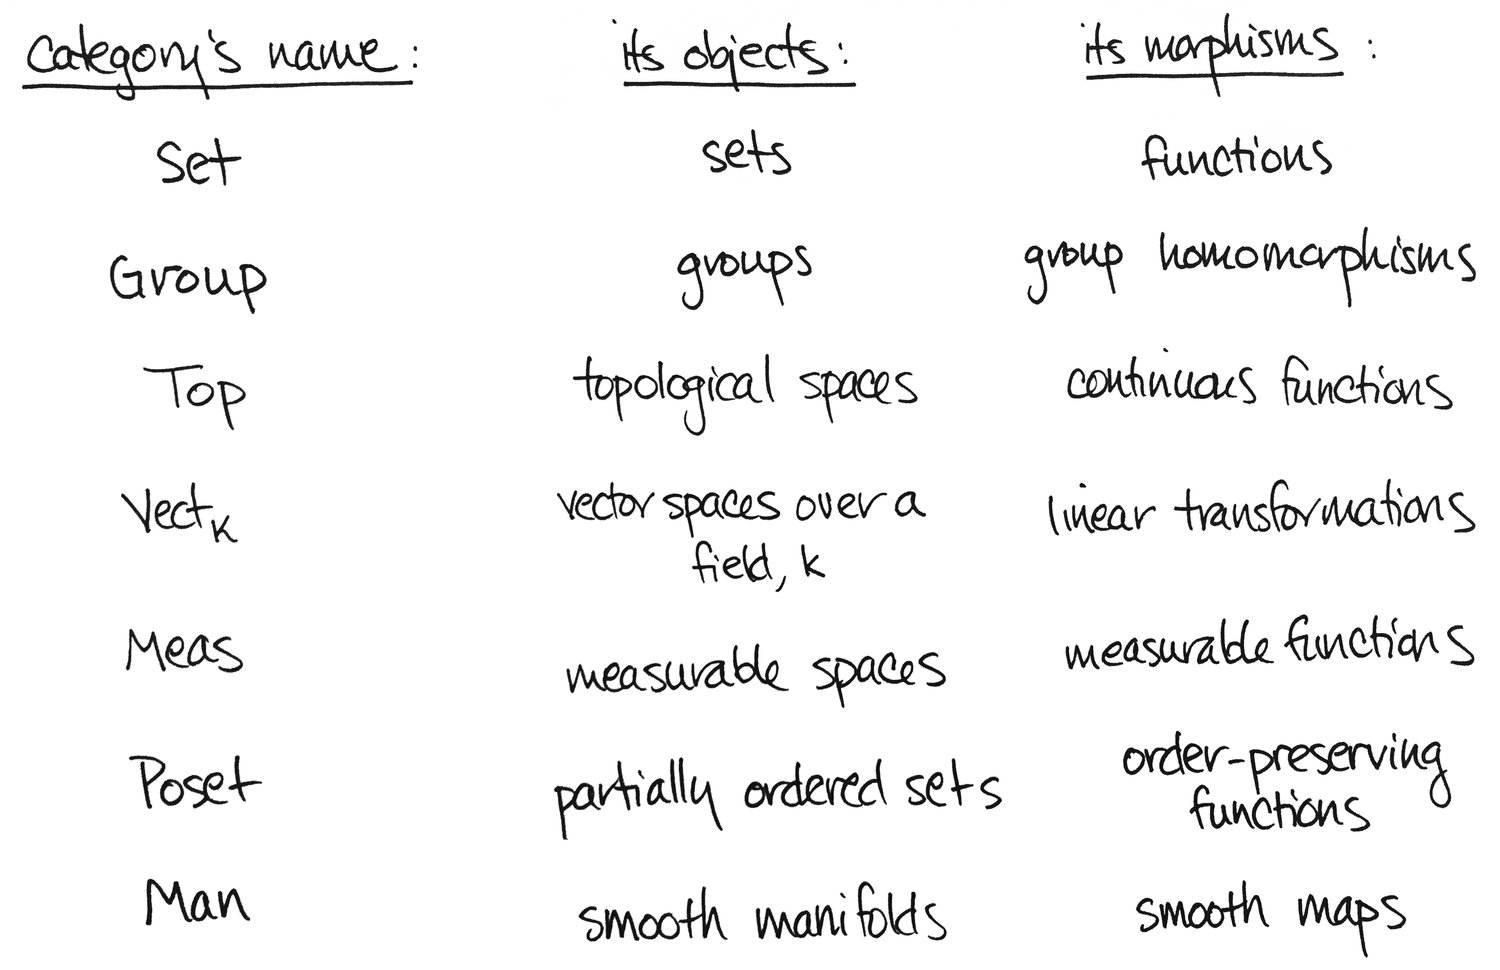
\includegraphics[width=10cm]{images/m2_categorytheory_intro.jpg}
\caption{\small{Examples of categories and morphisms defined in Category Theory \cite{categorytheory_intro}}}
\label{img:m2_category_theory_intro}
\end{figure}

The necessity of category theory for the project is to understand the fundamental groups (will be defined in Section \ref{sec:m2_fundamental_groups}) which require \newword{functors} -- maps between categories -- when we discuss the fundamental group functor \fgrp.

\section{Homotopy Theory}
\label{sec:m2_homotopy_theory}
For this section, let $I$ denote the unit interval. Let \topspace{X} and \topspace{Y} be topological spaces. Lastly, let $Cts(X,Y)$ denote the continuous functions from $X$ to $Y$.

\subsection{Homotopies}
\begin{keyterm}{Homotopic}
Let $f,g: \in Cts(X,Y)$. We say $f,g$ are \newword{homotopic} if there exists a continuous function $H: X \times I \to Y$ such that $H(x,0)=f(x)$ and $H(x,1)=g(x)\ \forall x \in X$. 
Think of it as a continuous deformation of $f$ into $g$ where the deformation itself is $H$. We denote $H$ as the \newword{homotopy} between the two continuous functions (note homotopies are not unique).
\end{keyterm}

\begin{keyterm}{Null-homotopic}
Let $f \in Cts(X,Y)$. We say $f$ is \newword{null-homotopic} if it is homotopic to a constant function.
\end{keyterm}

\begin{theorem}
Homotopy is an equivalence relation on $Cts(X,Y)$
\end{theorem}
\begin{proof}
Let $f,g,h \in Cts(X,Y)$.

\underline{Reflexive}:
Define $F = X \times I \to Y$ where $F(x,t) = f(x)$. It follows that $F$ is a homotopy from $f$ to $f$. Note $F$ is continuous as $f$ is.

\underline{Symmetric}:
Suppose $f$ homotopic to $g$ with homotopy $F$. Define $G: X \times I \to Y$ as $G(x,t) = F(x,1-t)$. Follows that $G$ is a homotopy of $g$ to $f$.

\underline{Transitive}:
Suppose $f,g$ and $g,h$ homotopic with homotopies $F$ and $H$, respectively. Define the function $G: X \times I \to Y$ as follows

\begin{equation*}
    G(x,t) =
    \begin{cases}
    F(x,2t) & 0 \leq t \leq 1/2\\
    H(x,2t-1) & 1/2 < t \leq 1
    \end{cases}
\end{equation*}

where it can be inspected that $G$ is continuous (even at $t=1/2$) which can be verified by the pasting lemma and that $G(x,0)=F(x,0)=f(x)$ and $G(x,1)=H(x,1)=h(x)$. Hence, we have $G$ is a homotopy of $f,h$.
\end{proof}

Following this, let the equivalence relation of homotopy of continuous functions on topological spaces be denoted by $\sim_{h}$. In addition, let $[f]_{\sim_{h}} = \{g \in Cts(X,Y) : f \sim_{h} g\}$ represent the equivalence class of $f$ for homotopy.


\begin{theorem}
Let $f,f' \in Cts(X,Y)$ and $g,g' \in Cts (Y,Z)$. If $f \sim_{h} f'$ and $g \sim_{h} g'$, then $(g \circ f) \sim_{h} (g' \circ f)$.
\end{theorem}
\begin{proof}
Let $F$ and $G$ be the homotopy for $f,f'$ and $g,g'$, respectively. Define $H: X \times I \to Z$ as $H(x,t) = G \circ (F(x,t),t)$. We note that $H$ is continuous because it is the composition of continuous functions. Then $H(x,0) = g \circ f(x)$ and $H(x,1) = g' \circ f'(x)$. Hence, $H$ is a homotopy between $g \circ f$ and $g' \circ f'$.
\end{proof}

\subsection{Homotopy Equivalence}

\begin{keyterm}{Homotopy equivalence}
Let $f \in Cts(X,Y)$ where $f$ is said to be a \newword{homotopy equivalence} of $X$ to $Y$ if there exists $g \in Cts(Y,X)$ s.t. $f \circ g \sim_{h} Id_{Y}$ and $g \circ f \sim_{h} Id_{X}$. In this sense, $g$ is denoted as the \newword{homotopy inverse} of $f$.
\end{keyterm}

\begin{keyterm}{Homotopy equivalent}
$X,Y$ are said to be \newword{homotopy equivalent} if there exists a homotopy equivalence $f \in Cts(X,Y)$. 
\end{keyterm}

\begin{theorem}
Homotopy equivalence is an equivalence relation on topological spaces.
\end{theorem}
\begin{proof}
\underline{Reflexive}:
Take the identify map as both homotopy equivalence and homotopy inverse on $X$ to $X$; hence, $X \sim X$.

\underline{Symmetric}:
Suppose $f \in Cts(X,Y)$ is a homotopy equivalence of $X$ to $Y$ with homotopy inverse $g$; that is $X \sim Y$. Follows that $g$ is a homotopy equivalence of $Y$ to $X$ with homotopy inverse $f$ i.e. $Y \sim X$.

\underline{Transitive}:
Suppose \topspace{Z} is a topological space as well where we have $X \sim Y$ and $Y \sim Z$. Hence, there exists functions $f_{1}, g_{1}, f_{2}, g_{2}$ as follows in the figure below where $f_{1}$ is a homotopy equivalence of $X$ to $Y$ with homotopy inverse $g_{1}$. Similarly, we have the relationship of $f_{2}$ and $g_{2}$ between $Y$ and $Z$.

\begin{figure}[H]
\centering
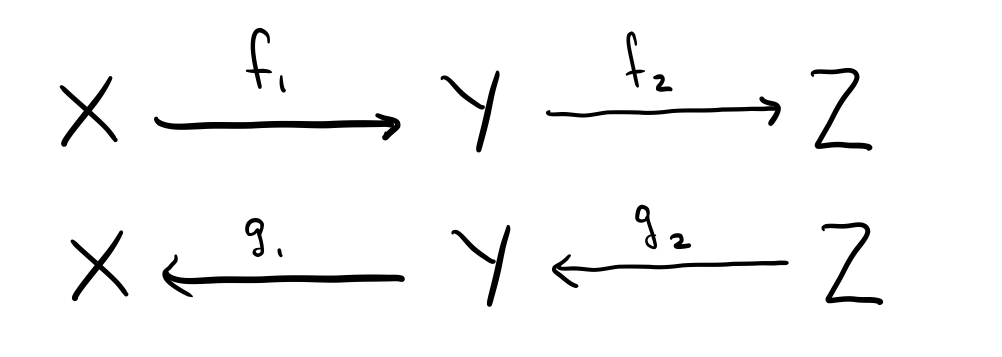
\includegraphics[width=10cm]{images/m2_homotopyequivalent_transitivity.png}
\end{figure}

Hence, we have $f_{1} \circ g_{1} \sim_{h} Id_{Y}$, $g_{1} \circ f_{1} \sim_{h} Id_{X}$ and $f_{2} \circ g_{2} \sim_{h} Id_{Z}$, $g_{2} \circ f_{2} \sim_{h} Id_{Y}$. Let $f = f_{2} \circ f_{1}$ and $g = g_{1} \circ g_{2}$. The claim is that $f$ is a homotopy equivalence of $X \to Z$ with homotopic inverse $g$, thereby showing that $X \sim_{h} Z$. We note that $f \circ g: Z \to Z$.

Define $H: Z \times I \to Z$ as follows:

\begin{equation*}
    H(z,t) =
    \begin{cases}
    f_{2} \circ H_{1}(y,2t) \circ g_{2}(z) & 0 \leq t \leq 1/2\\
    H_{2}(z,2t-1) & 1/2 < t \leq 1
    \end{cases}
\end{equation*}

where $H_{1}$ and $H_{2}$ are the homotopies of $f_{1} \circ g_{1}$ and $Id_{Y}$ and $f_{2} \circ g_{2}$ and $Id_{Z}$, respectively. We note that $H$ is a continuous function in both the cases as $H$ is the composition of continuous functions. At $t=1/2$, we note that both cases of $H$ assume the same value presented by $f_{2} \circ g_{2}$.

Based on this construction, $H(z,0) = f \circ g$ and $H(z,1) = Id_{Z}$. Hence, $H$ is a homotopy of $f \circ g$ and $Id_{Z}$ so $f \circ g \sim_{h} Id_{Z}$. Similarly, we can show that $g \circ f \sim_{h} Id_{X}$. Thus, $X \sim Z$.
\end{proof}

Following this, let the equivalence relation of homotopy equivalence between topological spaces be denoted by $\sim_{heq}$.

\begin{keyterm}{Contractible}
Let \topspace{X} be a topological space. $X$ is said to be \newword{contractible} if it is homotopy equivalent to a single point i.e. $X \sim_{heq} \{x_{0}\}$.
\end{keyterm}

\subsection{Category: Homotopy equivalent topological spaces}
Let $hTop$ represent this category as follows:

Denote $Obj(hTop) = Obj(Top) \slash_{X \sim Y}$ where $X$ and $Y$ are homotopy equivalent. 

Denote $Mor(hTop) = Mor(Top) \slash_{f \sim g}$ where $f,g: X \to Y$ are continuous functions that are homotopic.

To make the notion of functors more concrete, let F be a functor between the category of topological spaces to groups. If $f,g \in Mor(hTop)$ where recall that $f \circ g \in Mor(hTop)$, then $F(f \circ g) = F(f) \circ F(g)$ for $F(f), F(G) \in Mor(Group)$. Note that $F(f), F(g)$ are hence group homomorphisms under the morphisms of the category group.

\section{Fundamental Groups}
This section has been inspired by the notes of \cite{riemann_surfaces_algebraic_curves}.
\label{sec:m2_fundamental_groups}

\begin{keyterm}{Pointed topological space}
A \newword{pointed topological space} is a topological space with a \newword{basepoint} $x_{0}$.
\end{keyterm}

\begin{keyterm}{Fundamental Group}
The \newword{fundamental group} $\pi_1(X, x_0)$ of a pointed topological space $(X, x_0)$ is a group formed with the \emph{set of equivalence classes} with the equivalence relation $\sim_h$ of loops at the basepoint $x_0$; that is, continuous functions $$\gamma: [0, 1] \to (X, x_0)$$ such that $$\gamma(0)=\gamma(1)=x_0.$$
\end{keyterm}

\begin{keyterm}{Concatenation $*$ of based loops}
For $\gamma_1, \gamma_2$ loops at a basepoint $x_0$, define $\gamma_1 * \gamma_2$ as the loop in $X$ at $x_0$ defined by 

\begin{equation*}
    \gamma_1 * \gamma_2(s) =
    \begin{cases}
    \gamma_1(2s) & 0 \leq t \leq 1/2\\
    \gamma_2(2s-1) & 1/2 \leq t \leq 1
    \end{cases}
\end{equation*}

The \newword{concatenation} of based loops $\gamma_1, \gamma_2$ at $x_0 \in X$ is defined as $\gamma_1 * \gamma_2$.
\end{keyterm}

\begin{lemma}
\label{lem:m2_concatenation_preserves_homotopy}
The operation of concatenation of loops is compatible with homotopy equivalence of based loops. In other words, if $\gamma_1 \sim_h \psi_1$ and $\gamma_2 \sim_h \psi_2$, then $(\gamma_1 * \gamma_2) \sim_h (\psi_1 * \psi_2)$.
\end{lemma}

\begin{proof}
Let $H_1, H_2$ be the homotopies of $\gamma_1, \psi_1$ and $\gamma_2, \psi_2$, respectively. Define $H: [0,1] \times [0,1] \to X$ as 

\begin{equation*}
    H(s,t) =
    \begin{cases}
    H_1(2s,t) & 0 \leq t \leq 1/2\\
    H_2(2s-1,t) & 1/2 \leq t \leq 1
    \end{cases}
\end{equation*}

where $H$ is a homotopy between $(\gamma_1 * \gamma_2)$ and $(\psi_1 * \psi_2)$.
\end{proof}

\begin{keyterm}{Homotopy with respect to basepoint}
Let $x_0$ be a basepoint of $X$. Define loops $\gamma, \psi$ at $x_0$. We say that $\gamma$ and $\psi$ are \newword{homotopic w.r.t basepoint} if there exists a homotopy $H: [0,1] \times [0,1] \to X$ with the property that $H(0,t)=H(1,t)=x_0, \forall t \in [0,1]$. In other words, the basepoint $x_0$ is fixed in the the entire motion of the homotopy $H$ across the time interval. 
\end{keyterm}

\begin{claim}
Let \topspace{X} be a topological space and fix $x \in X$. Show that $\pi_{1}(X,x)$ is in fact a group with the binary operation of concatenation.
\end{claim}
\begin{proof}
For simplicity's sake, denote the equivalence class of homotopy as $[\_\_] = [\_\_]_{\sim_h}$. By Lemma \ref{lem:m2_concatenation_preserves_homotopy}, we have that $*$ induces an operation on the sets of the quotient set: given two equivalence classes of based loops $[\gamma_1], [\gamma_2]$, we have that $[\gamma_1]*[\gamma_2] = [\gamma_1 * \gamma_2]$. Hence, we have a well-defined binary operation and that the set of equivalence classes is in fact closed under concatenation. Now, we show the group axioms are held. 

\underline{Associativity}\\
Let $\gamma_1, \gamma_2, \gamma_3$ be loops based at $x_0 \in X$. We want to show that $([\gamma_1]*[\gamma_2])*[\gamma_3]=[\gamma_1]*([\gamma_2]*[\gamma_3])$. To do this, we will show $(\gamma_1*\gamma_2)*\gamma_3 \sim_h \gamma_1*(\gamma_2*\gamma_3)$. By the definition of concatenation, we note that the LHS loop is defined as 

\begin{equation*}
    (\gamma_1*\gamma_2)*\gamma_3 =
    \begin{cases}
    \gamma_1(4s) & 0 \leq s \leq 1/4\\
    \gamma_2(4s-1) & 1/4 \leq s \leq 1/2\\
    \gamma_3(2s-1) & 1/2 \leq s \leq 1
    \end{cases}
\end{equation*}

and the RHS as 

\begin{equation*}
    \gamma_1*(\gamma_2*\gamma_3) =
    \begin{cases}
    \gamma_1(2s) & 0 \leq s \leq 1/2\\
    \gamma_2(4s-2) & 1/2 \leq s \leq 3/4\\
    \gamma_3(4s-3) & 3/4 \leq s \leq 1
    \end{cases}
\end{equation*}

Now we define $H: [0,1] \times [0,1] \to X$ as follows:
\begin{equation*}
    H(s,t) =
    \begin{cases}
    \gamma_1(\frac{4s}{t+1}) & 0 \leq s \leq \frac{t}{4} + \frac{1}{4}\\
    \gamma_2(4s-(1+t)) & \frac{t}{4} + \frac{1}{4} \leq s \leq \frac{t}{4} + \frac{1}{2}\\
    \gamma_3(2s+t(2s)-1+t(-2)) & \frac{t}{4} + \frac{1}{2} \leq s \leq 1
    \end{cases}
\end{equation*}

where by cleaning up $H$, it follows that
\begin{equation*}
    H(s,t) =
    \begin{cases}
    \gamma_1(\frac{4s}{t+1}) & 4s-1 \leq t\\
    \gamma_2(4s-(1+t)) & 4s-2 \leq t \leq 4s-1\\
    \gamma_3(2s(t+1)-(1+2t)) & t \leq 4s-2
    \end{cases}
\end{equation*}

where it can be see that $H(s,0) = (\gamma_1*\gamma_2)*\gamma_3$ and $H(s,1) = \gamma_1*(\gamma_2*\gamma_3)$ and $H$ is a continuous map. Thus, $H$ is a homotopy and that $([\gamma_1]*[\gamma_2])*[\gamma_3]=[\gamma_1]*([\gamma_2]*[\gamma_3])$.

\underline{Identity}\\
Let $\gamma$ be a loop defined at a basepoint $x_0 \in X$. Define the constant map $e_{x_0}$ as $e_{x_0}(s) = x_0, \forall s \in [0,1]$. We want to show that $\gamma * e_{x_0} \sim_h \gamma$. We note that 

\begin{equation*}
    \gamma * e_{x_0} =
    \begin{cases}
    \gamma(2s) & s \in [0,\frac{1}{2}]\\
    x_0 & s \in [\frac{1}{2}, 1]
    \end{cases}
\end{equation*}

Define the function $H:[0,1] \times [0,1] \to X$ as follows:

\begin{equation*}
    H(s,t) =
    \begin{cases}
    \gamma(\frac{2s}{t+1}) & 0 \leq s \leq \frac{t}{2} + 1/2 \Leftrightarrow 2s-1 \leq t\\
    x_0 & \frac{t}{2} + \frac{1}{2} \leq s \leq 1 \Leftrightarrow t \leq 2s-1
    \end{cases}
\end{equation*}

Note that $H$ is a homotopy between the $e_{x_0} * \gamma$ and $\gamma$. We note that a very similar argument can be employed to identify a homotopy between $\gamma * e_{x_0}$ and $\gamma$, which would then showcase that $[\gamma]*[e_{x_0}] = [e_{x_0}]*[\gamma] = [\gamma]$. Hence, $[e_{x_0}]$ is the identity of the set of equivalence classes under concatenation.

\underline{Inverse}\\
Let $\gamma$ be a loop defined at a basepoint $x_0 \in X$. Given $[\gamma]$, we have $[\gamma]^{-1} = [\gamma^{-1}]$ where $\gamma^{-1}(s) = \gamma(1-s)$. Informally, $\gamma^{-1}$ is the loop $\gamma$ but in the "reverse direction" or "other way around". We want to show that $[\gamma * [\gamma^{-1}] = [e_{x_0}]$. In other words, we want to show there exists a homotopy between $\gamma * \gamma^{-1}$ and $e_{x_0}$. By defining the function $H:[0,1] \times [0,1] \to X$ as follows:

\begin{equation*}
    H(s,t) =
    \begin{cases}
    \gamma(s) & 0 \leq s \leq \frac{t-1}{2}\\
    \gamma(\frac{1-t}{2}) & \frac{t-1}{2} \leq s \leq \frac{t+1}{2}\\
    \gamma^{-1}(s) & \frac{t+1}{2} \leq s \leq 1
    \end{cases}
\end{equation*}

Note similarly, we may show that $[\gamma^{-1}]*[\gamma] = [e_{x_0}]$.

The pair $\pi_1(X,x_0)$ is thus a fundamental group defined with the binary operation of concatenation.
\end{proof}

\mainpoint{$\pi_{1}$ is a \newword{covariant} functor. This means that, given \topspace{X} and \topspace{Y}, and a $f \in Cts(X,Y)$, $f_*: \pi_{1}(X)\to\pi_{1}(Y)$ is a group homomorphism where $f_*$ can be thought of as $\pi_{1}(f)$.}

For basepoints $x_0 \in X$ and $f(x_0) \in Y$. We define $\pi_{1}(f)$ between the fundamental groups of $\pi_{1}(X,x_0)$ and $\pi_{1}(Y,y_0)$ as follows:
 
\begin{align*}
    \pi_{1}(f): \pi_{1}(X,x_0) &\to \pi_{1}(Y,f(x_0))\\
    [\gamma] &\mapsto [f \circ \gamma]
\end{align*}

We denote $f_*$ = $\pi_{1}(f)$ as the \emph{induced homomorphism} of the map $f$.

\begin{claim}
\label{claim:m2_fgrp_exercises}
Let $f \in Cts(X,Y)$ and $g \in Cts(Y,Z)$ sending $x_0 \mapsto y_0 \mapsto z_0$. Prove that:

(a) \underline{$\pi_{1}(f): \pi_{1}(X,x_0) \to \pi_{1}(X,y_0)$ is a group homomorphism}
\begin{proof}
Let $[\gamma], [\beta] \in \pi_{1}(X,x_0)$. 
\begin{align*}
    \pi_{1}(f)([\gamma]*[\beta]) &= \pi_{1}(f)([\gamma * \beta])\\
                            &= [f \circ (\gamma * \beta)]\\
\intertext{
where now we note that the following equation is identical for $f \circ (\gamma * \beta)$ and $(f \circ \gamma) * (f \circ \beta)$
\begin{equation*}
    \begin{cases}
    f \circ \gamma(2s) & 0 \leq s \leq \frac{1}{2}\\
    f \circ \beta(2s-1) & \frac{1}{2} \leq s \leq 1
    \end{cases}
\end{equation*}
Hence,
}
    \pi_{1}(f)([\gamma]*[\beta]) &= [(f \circ \gamma) * (f \circ \beta)]\\ 
                            &= [(f \circ \gamma)] * [(f \circ \beta)]\\
                            &= \pi_{1}(f)([\gamma]) * \pi_{1}(f)([\beta])
\end{align*}
\end{proof}
\pagebreak

(b) \underline{$\pi_1{Id_X} = Id_{\pi_{1}(X,x_0)}$}
\begin{proof}
Let $[\gamma] \in \pi_{1}(X,x_0)$.
\begin{equation*}
    \pi_{1}(Id_X)([\gamma]) = [Id_X \circ \gamma]
                            = [\gamma]
                            = Id_{\pi_{1}(X,x_0)}([\gamma])
\end{equation*}
\end{proof}

(c) \underline{$\pi_{1}(g \circ f) = \pi_{1}(g) \circ \pi_{1}(f)$}
\end{claim}
\begin{proof}
Let $[\gamma] \in \pi_{1}(X,x_0)$.
\begin{equation*}
    \pi_{1}(g \circ f)([\gamma]) = [(g \circ f) \circ \gamma]
                            = [g \circ (f \circ \gamma)]\\
                            = (\pi_{1}(g))([f \circ \gamma])
                            = (\pi_{1}(g))((\pi_{1}(f))([\gamma]))
                            = (\pi_{1}(g) \circ \pi_{1}(f))([\gamma])
\end{equation*}    
\end{proof}

\begin{claim}
Let $(X,x_0), (Y,y_0)$ be homeomorphic pointed topological spaces. Then $\pi_{1}(X,x_0) \isom \pi_{1}(Y,y_0)$
\end{claim}
\begin{proof}
For $(X,x_0), (Y,y_0)$ to be homeomorphic, there must exist $f \in Cts(X,y)$ and $g \in Cts(Y,X)$ such that $f \circ g = Id_Y, g \circ f = Id_X, f(x_0)=y_0$. We want to show that $\pi_{1}(f)$ is a group isomorphism with $\pi_{1}(g)$ as the inverse between $\pi_{1}(X,x_0)$ and $\pi_{1}(Y,y_0)$. We note that by Claim \ref{claim:m2_fgrp_exercises}, it follows
\begin{equation*}
    \pi_{1}(g) \circ \pi_{1}(f) = \pi_{1}(g \circ f) = \pi_{1}(Id_X) = Id_{\pi_{1}(X,x_0)}
\end{equation*}
Similarly, $\pi_{1}(f) \circ \pi_{1}(g) = Id_{\pi_{1}(Y,y_0)}$. Hence, $\pi_{1}(X,x_0) \isom \pi_{1}(Y,y_0)$.
\end{proof}

\begin{theorem}
Let \topspace{X} be a topological space. If $X$ is path connected, then for any two pairs of points $x_0,x_1 \in X, \pi_{1}(X,x_0) \isom \pi_{1}(X,x_1)$.
\end{theorem}
\begin{proof}
Let $f \in Cts(X,X)$ where $f(x_0) = x_1$. Let $[\gamma]$ denote the homotopy class of paths that begin at $x_1$ and end at $x_0$. Define the function as follows
\begin{align*}
    \psi(\delta): \pi_{1}(X,x_0) &\to \pi_{1}(X,x_1)\\
    [\delta] &\mapsto [\gamma \delta \gamma^{-1}]
\end{align*}

where $[\delta] \in \pi_{1}(X,x_0)$. That is, $[\delta]$ represents an equivalence class of loops based at $x_0$. Let $[\beta]$ represent another such class. First we note that 
\begin{align*}
\psi(\delta\beta) &= [\gamma(\delta\beta)\gamma^{-1}]\\
                    &= [\gamma\delta\gamma^{-1}\gamma\beta\gamma^{-1}]\\
                    &= [\gamma\delta\gamma^{-1}][\gamma\beta\gamma^{-1}]\\
                    &= \psi(\delta)\psi(\beta)
\end{align*}
So indeed, $\psi$ is a group homomorphism. Now we want to show it is in fact an isomorphism.

Note that if $\psi(\delta) = [\gamma \delta \gamma^{-1}] = [\gamma \beta \gamma^{-1}] = \psi(\beta)$, it follows that $[\delta]=[\beta]$. Hence, $\psi$ is injective.

Let $[\delta] \in \pi_{1}(X,x_1)$. Then we note that $[\gamma^{-1} \delta \gamma] \in \pi_{1}(X,x_0)$ and so clearly $[\delta]$ is in the image of $\psi$ so $\psi$ is surjective. Thus, $\psi$ is an isomorphism.
\end{proof}
Note that the isomorphism is \emph{non-canonical} as it depends on the path $\delta$. Note that if the space $X$ is simply connected, then the isomorphism defined between fundamental groups of two basepoints is canonical.
\pagebreak

\begin{corollary}
Let \topspace{X} be a topological space. If $X$ is path connected, we unambiguously associate $X$ with a single fundamental group given by $\pi_{1}(X)$.
\end{corollary}

\begin{theorem}
Let \topspace{X} and \topspace{Y} be topological spaces where $X,Y$ are path connected. If $X \sim_{heq} Y$, $\pi_{1}(X) \isom \pi_{1}(Y)$.
\end{theorem}
\begin{proof}
Since $X$ and $Y$ are homotopy equivalent, there exists functions $f \in Cts(X,Y)$ and $g \in Cts(Y,X)$ where $g \circ f \sim_h Id_X$ and $f \circ g \sim_h Id_Y$. Let $x_0 \in X$ be a basepoint of $X$. Select $f(x_0)=y_0 \in Y$ as a basepoint of $Y$.

Let $[\gamma] \in \pi_{1}(X,x_0)$. Let $f_*: \pi_{1}(X,x_0) \to \pi_{1}(Y,y_0)$ be the induced homomorphism of $f$. Similarly, $g_*: \pi_{1}(Y,y_0) \to \pi_{1}(X,x_0)$. By Claim \ref{claim:m2_fgrp_exercises}, we have that $g_*, f_*$ are group homomorphisms. The claim is that $f_*$ and $g_*$ are inverses of one another. 

\begin{equation*}
    (g \circ f)_* = g_* \circ f_* = (Id_X)_* = Id_{\pi_{1}(X,x_0)}
\end{equation*}

Similarly, we have $(f \circ g)_* = Id_{\pi_{1}(Y,y_0)}$. Through this manner, we identify that the homomorphisms of of $f_*, g_*$ are inverses of one another and so $\pi_{1}(X,x_0)$ and $\pi_{1}(X,y_0)$ are isomorphic to each other.
\end{proof}

\begin{keyterm}{Isotopy}
For distinction, recall that a homotopy is simply a deformation between maps that involves shrinking, bending, and stretching i.e. is a deformation between continuous functions through continuous functions. The homotopy does not necessarily have to be surjective or injective, but that property is required by an isotopy.

An \newword{isotopy} is stricter in the sense that it is a continuous deformation of homeomorphisms between two \emph{homeomorphisms} and hence only involves bending; hence, at every $t \in [0,1]$, the isotopy between two homeomorphisms must be a homemorphism as well. Note that this also showcases that the two homeomorphisms are homotopic.
\end{keyterm}

% MEETING 3
\lecture{3}{Covering Maps and Universal Covers}{May 10th}{Drimik Roy}
\setcounter{section}{0}
\section{Overview}
Tasks to complete:
\begin{enumerate}
    \item Understand a statement of the uniformization theorem.
    \item Define a covering map and a covering space, and understand the path lifting property for maps.
    \item Define a deck transformation.
\end{enumerate}

\begin{keyterm}{Covering map and Covering space}
Let \topspace{X} and \topspace{Y} be topological spaces. A \newword{covering map} $p: X \to Y$ is a \emph{continuous, surjective map} such that $\forall y \in Y$ and for each $x_i \in p^{-1}(y)$, there exists a open \nghd $U_y$ of y where $p^{-1}(U_y)$ is a disjoint collection of open nghds $U_{x_i}$ i.e. $p^{-1}(U_y) = \bigdisjointunion_{x_i \in p^{-1}(y)} U_{x_i}$ and the restriction of $p$ on each of the neighborhoods $U_{x_i}$ in the disjoint collection is a \emph{homeomorphism} onto $U_y$.

$X$ here is the \newword{covering space}. Other key terms: Y is known as the \newword{base space} and the pre-image $p^{-1}(y)$ of some $y \in Y$ is known as the \newword{fiber over y}.
\end{keyterm}

\section{Notions of connectedness (continued)}
This section expands on concepts in Section \ref{sec:m2_connectedness}. For definitions, let \topspace{X} be a topological space. 

\begin{keyterm}{Locally connected}
$X$ is locally connected at $x \in X$ if $\forall\ V \in \tau_X$ containing $x$, there exists an open, connected set $U$ contained in $V$ i.e. $x \in U \subseteq V$. $X$ is said to be \newword{locally connected} if this is true $\forall x \in X$.
\end{keyterm}

\begin{keyterm}{Locally path connected}
$X$ is locally path connected at $x \in X$ if $\forall\ V \in \tau_X$ containing $x$, there exists an open, path-connected set $U$ contained in $V$ i.e. $x \in U \subseteq V$. $X$ is \newword{locally path connected} if this is true $\forall x \in X$.
\end{keyterm}

\begin{keyterm}{Locally simply connected}
$X$ is \newword{locally simply connected} if $\forall x \in X$ and $\forall V \in \tau_X$ containing $x$, there is an open set $U \subseteq V$ where $x \in U$ such that $U$ is simply connected in $X$. 

Every locally simply connected space is both locally connected and locally path connected.
\end{keyterm}

\begin{keyterm}{Semi-locally simply connected}
$X$ is \newword{semi-locally simply connected} if $\forall x \in X$, there exists a (\underline{should this be an open or closed}) \nghd $U$ containing $x$ where every loop in $U$ is contractible to a single point in $X$. Note that $U$ does not have to be simply connected as the loop might contract to a point outside of $U$.
\end{keyterm}

\section{Lifting properties}
\begin{keyterm}{Local homeomorphism}
$f \in Cts(X,Y)$ is called a \newword{local homeomorphism} if $\forall x \in X$, there exists a \nghd $U \subseteq X$ where $x \in U$ such that $f|_{U}: U \to f(U)$ is a homeomorphism onto an open subset of $f(U)$ of $Y$.
\end{keyterm}

Note that every covering map is a surjective local homeomorphism.

\begin{lemma}
A surjective local homemorphism is an open mapping. In particular, any covering map is an open mapping. 
\end{lemma}

This section is inspired by \cite{hatcher_algebraic_topology}.
\begin{keyterm}{Lift}
Let $p: X \to Y$ be a covering map. A \newword{lift} of a continuous map $\alpha: \tilde{X} \to Y$ is a continuous function $\tilde{\alpha}: \tilde{X} \to X$ where $p \circ \tilde{\alpha} = \alpha \forall x \in \tilde{X}$.
\end{keyterm}

\begin{figure}[H]
\centering
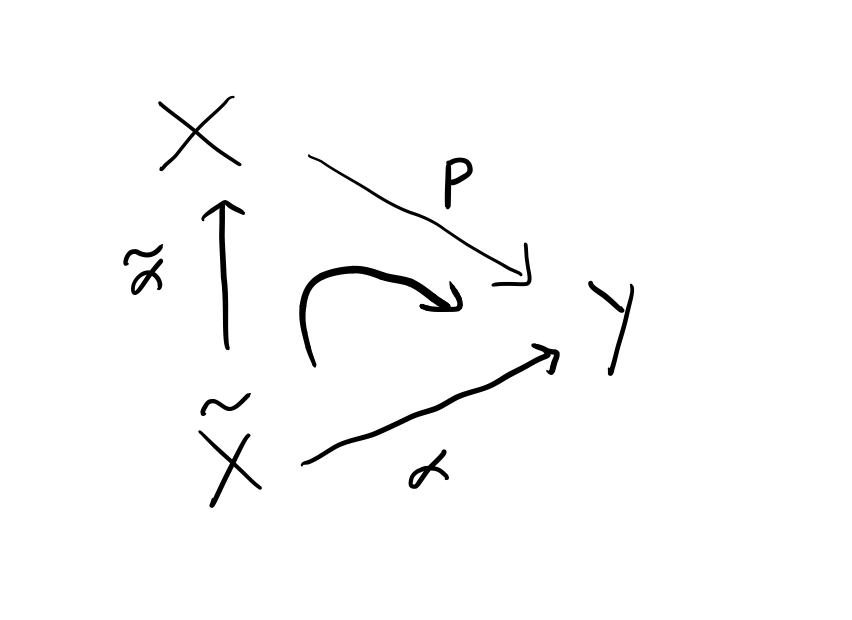
\includegraphics[width=10cm]{images/m3_lifting_diagram.png}
    \caption{\small{Diagram for Lifting}}
\label{img:m3_lifting_diagram}
\end{figure}

\begin{theorem}\newword{Uniqueness-of-lifting property}
We say $p: X \to Y$ has the uniqueness-of-lifting property if $\tilde{\alpha}_1, \tilde{\alpha}_2$ are two liftings of $\alpha$ where both $\tilde{\alpha}_1, \tilde{\alpha}_2$ agree on a single point i.e. $\tilde{\alpha}_{1}(z_0)=\tilde{\alpha}_{2}(z_0)$, then $\tilde{\alpha}_1 = \tilde{\alpha}_2$.
\end{theorem}

Now, when do paths in fact have a lift? At least covering maps always do (as covering maps are surjective local homeomorphisms and surjective local homeomorphims have the uniqueness-of-lifting property) and whenever an initial point is fixed, the lift is unique.

\begin{figure}[H]
\centering
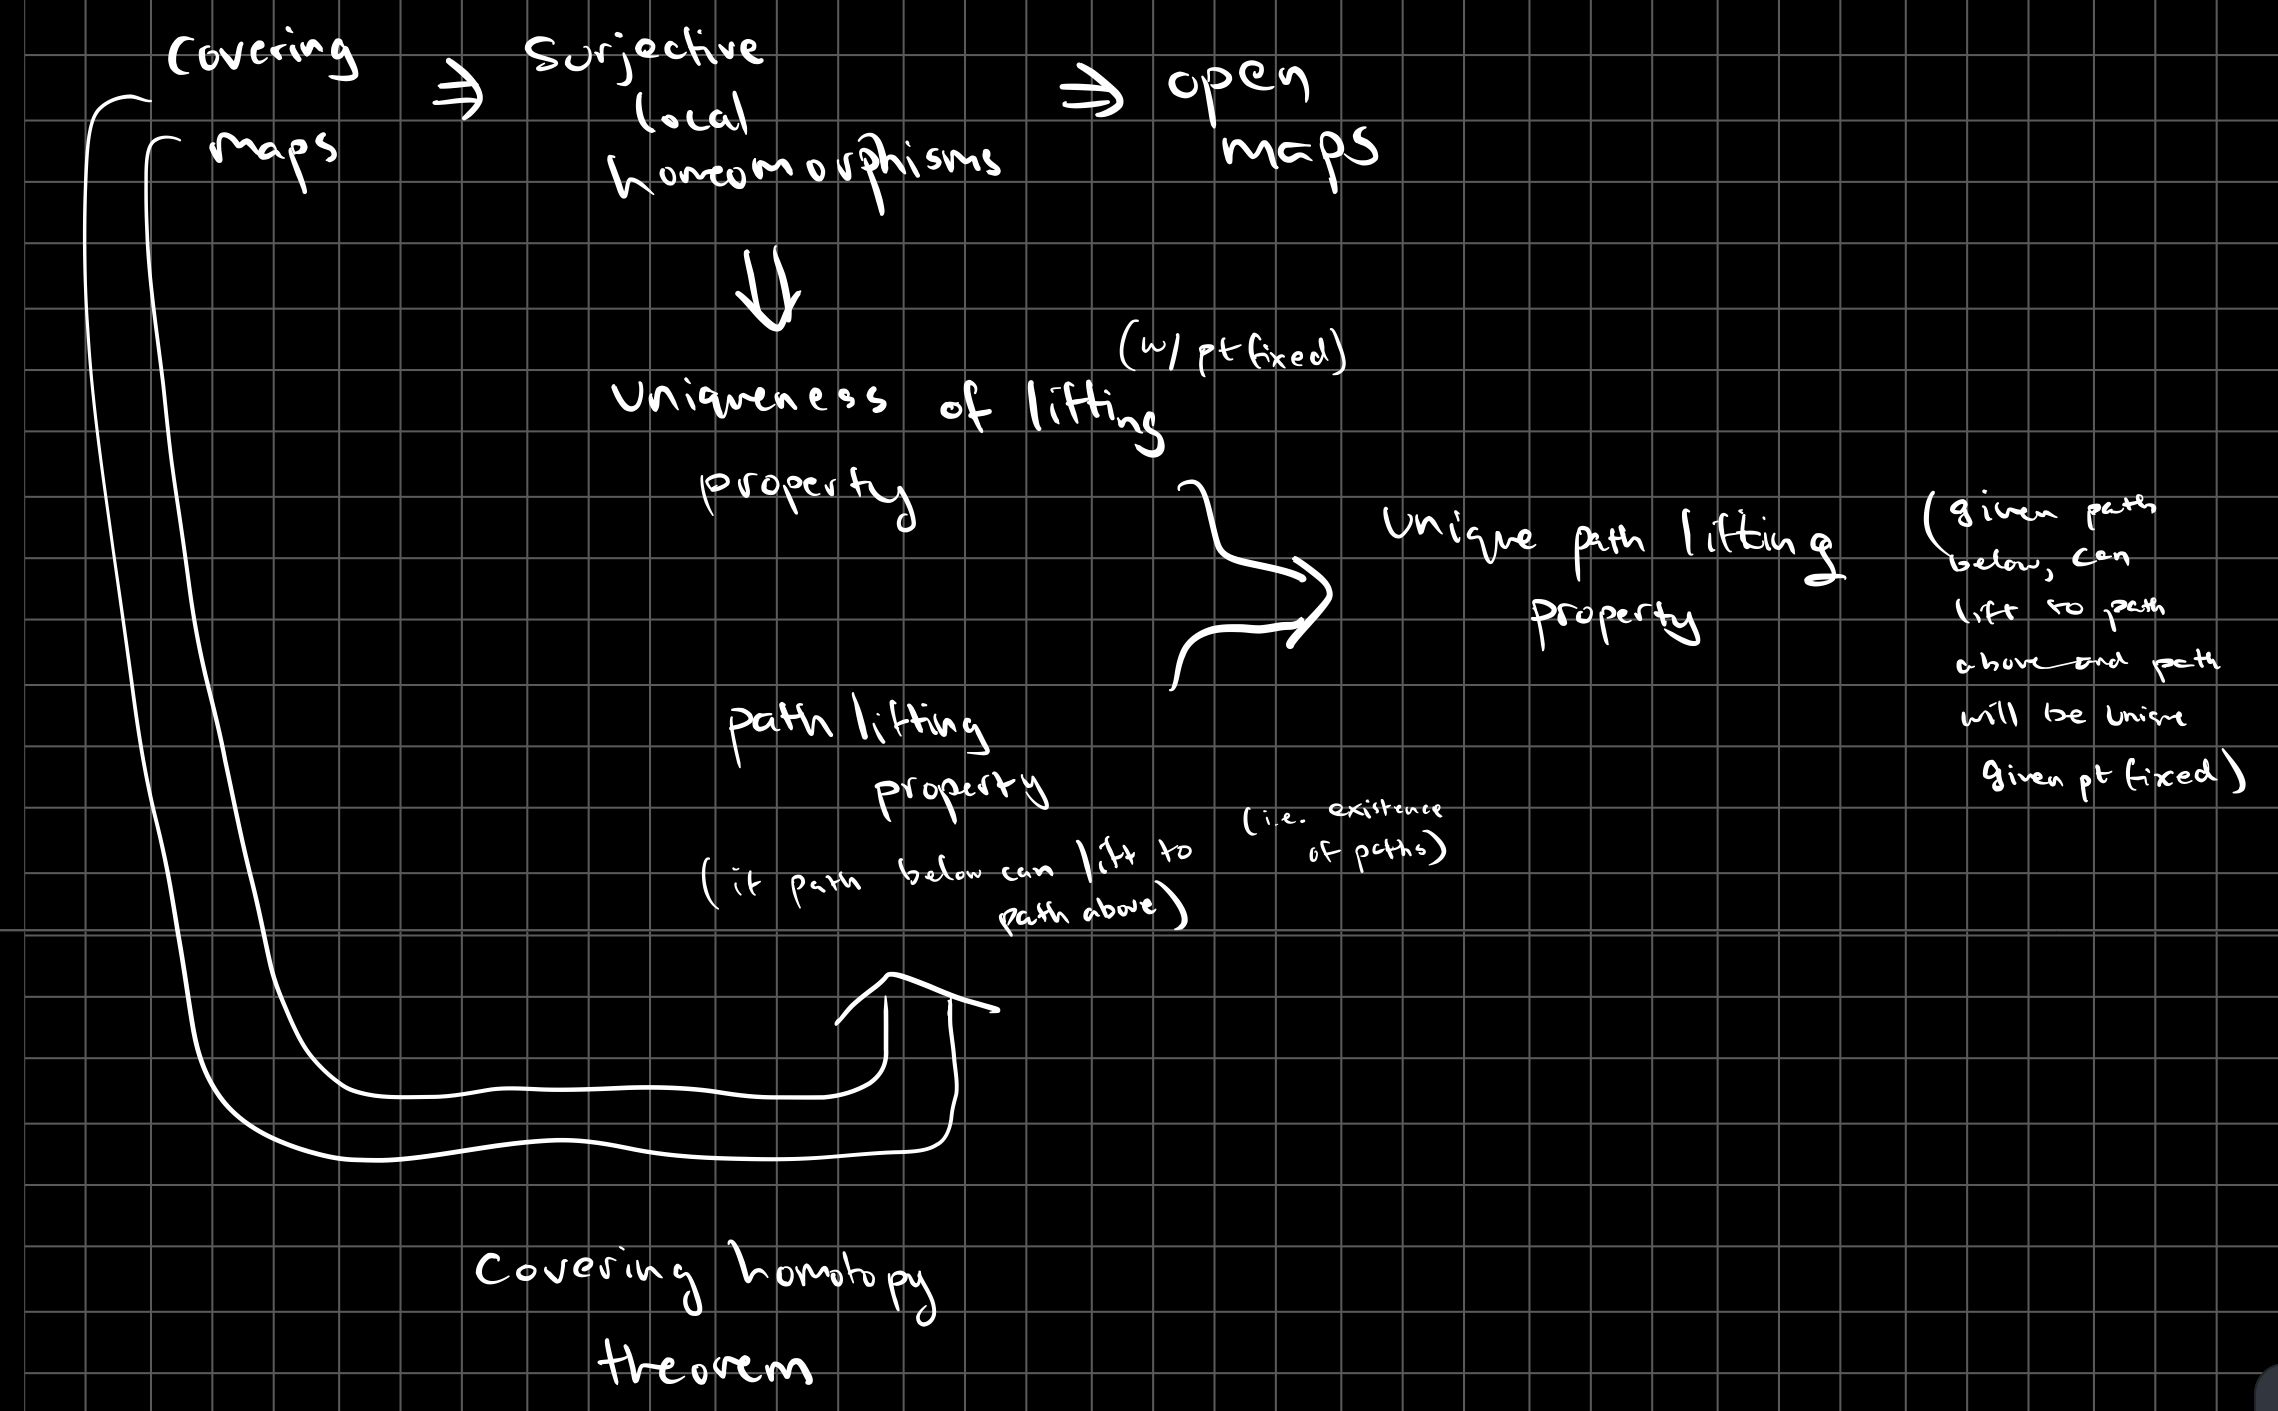
\includegraphics[width=\textwidth]{images/m3_covering_maps_implications.png}
    \caption{\small{Implications for covering maps}}
\label{img:m3_covering_maps_implications}
\end{figure}

\mainpoint{A surjective local homeomorphism with the path lifting property is a covering map.}

\subsection{Covering Homotopy Theorem}

\begin{figure}[H]
\centering
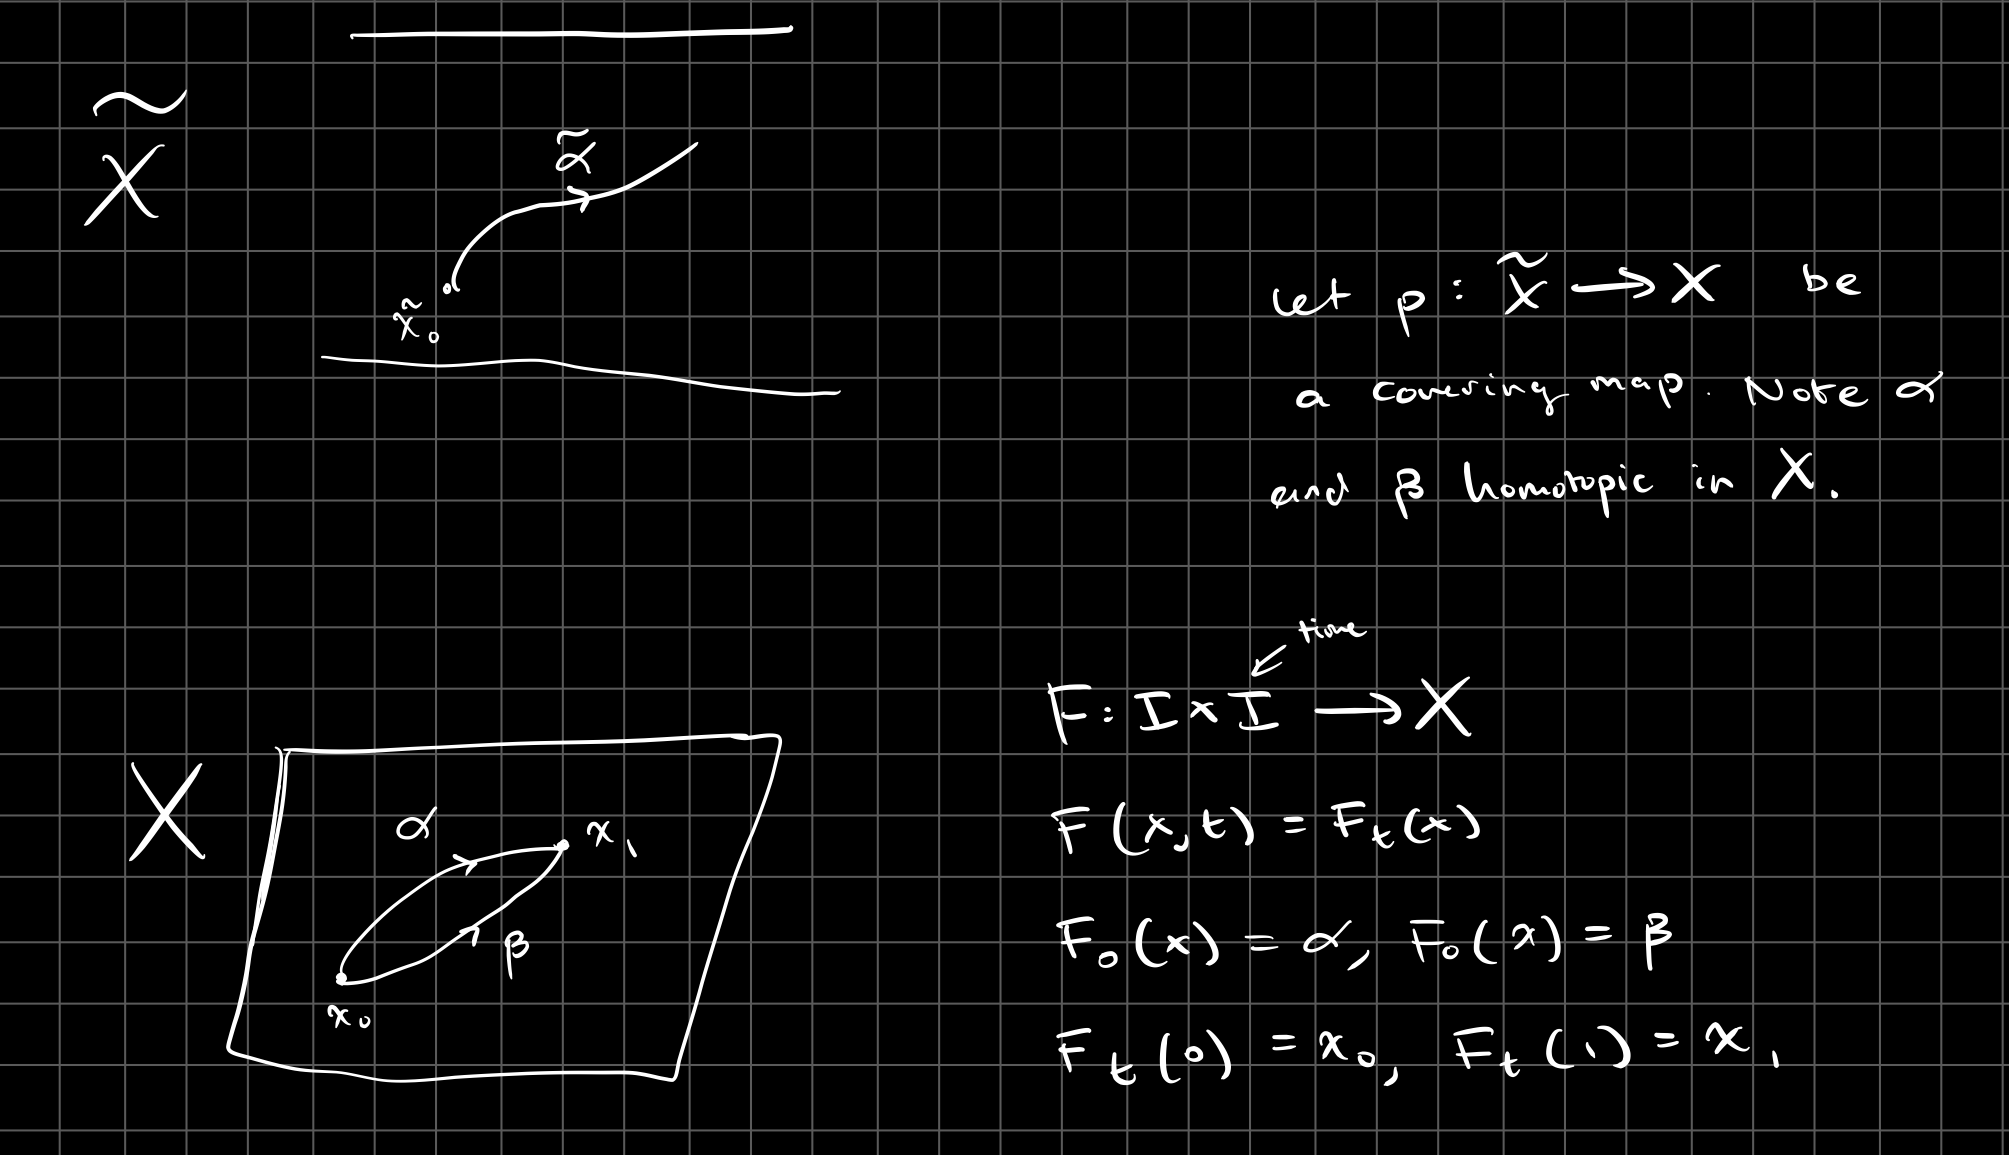
\includegraphics[width=12cm]{images/m3_covering_homotopy_theorem.png}
    \caption{\small{Covering Homotopy Theorem Case with Homotopy of Paths}}
\label{img:m3_covering_homotopy_theorem}
% https://www.youtube.com/watch?v=Yj6NRQIsZ-4
\end{figure}

We note that $\tilde{\alpha}$ is a lift of the path $\alpha$. 

\underline{Statement}: Given a homotopy of paths $F$ from $\alpha$ to $\beta$ in $X$ and given a lifting $\tilde{\alpha}$ of $\alpha$ to $\tilde{X}$ i.e. $p \circ \tilde{\alpha} = \alpha$, then we can find a homotopy $G: I \times I \to \tilde{X}$ which is a lifting of F with $G_{0}(x) = \tilde{\alpha}$ and in general, $G_{t}(x) = G(x,t)$.

We note the statement is a special case of the covering homotopy theorem with regards to paths. The general case deals with homotopy of \emph{continuous maps}.

Mainly, any homotopy $F: Z \times I \to X$ with \textbf{Z compact, connected, locally connected} can be lifted to a homotopy $G: Z \times I \to \tilde{X}$ with $G_t$ lying over $F_t$ for each $t \in I$.

\begin{figure}[H]
\centering
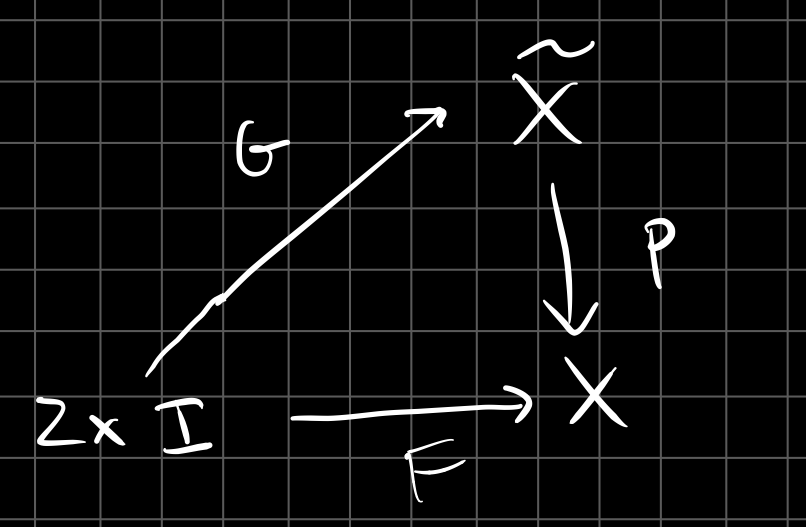
\includegraphics[width=10cm]{images/m3_general_covering_homotopy_theorem.png}
    \caption{\small{Diagram for general case for Covering Homotopy Theorem}}
\label{img:m3_general_covering_homotopy_theorem}
\end{figure}

\begin{lemma}
In particular, if $z \in Z$ with $F(z,t)$ is constant for some subinterval $J$ of $I$ with $t \in J$, then $G(z,t)$ is also constant for that subinterval.
\end{lemma}

\section{Relationship of fundamental group and covering spaces}
This section derives its notes from "Fundamental Groups and Connections to Covering Spaces" \cite{fundamental_groups_and_connections_to_covering_spaces}.

The notion of coverings is very important in the relationship between the fundamental group of the covering and base space.

\subsection{$\RR$ as a covering space of $S^1$}
First we shall begin with an exploration of the covering map $p: \RR \to S^1$. 
\begin{claim}
Let $p: \RR \to S^1$ as $p(x) = e^{ix} = (cos(x), sin(x))$. Show $p$ is an open map.
\end{claim}
\begin{proof}
Let $U$ be an open set in $\RR$. Define $X = S^{1} \setminus p(U)$. We want to show $X$ is closed. Note that $p^{-1}(p(U)) = U + 2 \pi n$ where $n \in \ZZ$ is open. Then its complement, which is $p^{-1}(T)$ is closed in $\RR$. Since $[0,2 \pi]$ is compact in $\RR$ and thus $p^{-1}(T) \intersection [0, 2 \pi]$ is compact in $\RR$. Because $p$ is surjective when restricted to $[0,2 \pi]$, we have that $T = p(p^{-1}(T) \intersection [0, 2 \pi]$ and so T is compact, thus T is closed. Hence, its inverse $p(U)$ is open.
\end{proof}
\pagebreak

\begin{claim}
Let $x \in \RR$. Show that $p|_{(x, x+2 \pi)}$ is a homeomorphism onto $S^{1} \setminus \{p(x)\}$.
\end{claim}
\begin{proof}
Clear that $p$ is bijective and continuous and $p^{-1}$ continuous by $p$ being an open map.
\end{proof}

We say that $p$ has the unique path lifting property that if we have a path $f$ in $S^1$ with $f(0) = p(s_0)$ with $s_0 \in \RR$, then there exists a unique lift $\tilde{f}: I \to \RR$ such that $\tilde{f}(0) = s_0$ and $p \circ \tilde{f} = f$. Once again the uniqueness of the lift is dependent on the initial value of $s_0$. This is important in the definition of when the path $f$ is a loop.

If $f$ is a loop, $f(0)=f(1)=p(s_0)$ and so $\tilde{f}(0) = s_0$ and thus $\tilde{f}(1) = s_0 + 2 \pi n$ where $n \in \ZZ$.

\begin{keyterm}{Winding number}
Let $f$ be a loop in $S^1$. The \newword{winding number} of $f$ is 
\begin{equation*}
    n(f) = \frac{\tilde{f}(1) - \tilde{f}(0)}{2\pi}
\end{equation*}
where $\tilde{f}$ is a lift of $f$.
\end{keyterm}

We note that any lift of $f$ to $S^1$ differs by an integer multiple of $2 \pi$.

\begin{lemma}
\label{lem:m3_winding_number_facts}
Let $f,g: I \to S^1$ be loops in $S^1$ with \emph{identical basepoint}. Then:\\
(a) $n(fg) = n(f) + n(g)$.\\
(b) If $f \sim_h g$, then $n(f) = n(g)$.\\
(c) If $n(f) = n(g)$, then $f \sim_h g$.\\
(d) Let $x \in S^1$. For all integers $k$, there exists a loop $h: I \to S^1$ based at $x$ such that $n(h) = k$.
\end{lemma}
\begin{proof}
Refer to \cite{fundamental_groups_and_connections_to_covering_spaces} pages 10 to 12.
\end{proof}

We note that by (b) and (c) we have that $f \sim_h g$ iff $n(f) = n(g)$.

\begin{theorem}
Show $\pi_{1}(S^1) \isom (\ZZ,+)$
\end{theorem}
\begin{proof}
We will refer to Lemma \ref{lem:m3_winding_number_facts} repeatedly.
Let $[f] \in \pi_{1}(S^1)$. By (b), we have that all loops in $[f]$ have the same winding number $\therefore n([f]) = n(f)$ well-defined. By (a), the map $[f] \mapsto n([f])$ defines a group homomorphism from $\pi_{1}(S^1)$ to $(\ZZ,+)$. With (c) and (d), the map is bijective. Thus, the map of winding number is an isomorphism between $\pi_{1}(S^1)$ and $(\ZZ,+)$.
\end{proof}

\begin{theorem}
Let $p: (\tilde{X},\tilde{x_0}) \to (X,x_0)$ be a covering space where $\tilde{x_0}$ is a fiber of $p^{-1}(x_0)$. Then the induced map $p_*: \pi_{1}(\tilde{X},\tilde{x_0}) \to \pi_{1}(X,x_0)$ is injective.
\end{theorem}
\begin{proof}
We will show that the kernel of $p_*$ is trivial. Let $[\gamma]$ be a homotopy class of based loops at $\tilde{x_0}$ where $p \circ \gamma \sim_h e_{x_0}$. By the homotopy lifting property, there exists a homotopy between $\gamma$ and $e_{\tilde{x_0}}$. Hence, $[e_{\tilde{x_0}}]=[\gamma]$, which is the identity, so $p_*$ is injective.
\end{proof}

% MEETING 4
\lecture{4}{MORE Covering Maps and Universal Covers}{May 10-17th}{Drimik Roy}
\setcounter{section}{0}
\section{Overview}
The goal of Week 2: May 13th - Math 17th is to understand the \emph{construction of Riemann surfaces} via quotient. 

Note the following implication statements: Locally connected $\Longrightarrow$ path connected $\Longrightarrow$ connected

\section{Examples of $\pi_1$}
\begin{enumerate}
    \item \underline{Contractible spaces}. i.e. $X \sim_{heq} {x_0}$ so $\pi_{1}(X) = \{e\}$.
    \item \underline{$S^n$ for $n \geq 2$}. $\pi_{1}(S^n) = \{e\}$. Note that $S^n$ is simply connected for $n \geq 2$.
    \item \underline{$S^1$}. $\pi_{1}(S^1) = \ZZ$.
    \item \underline{Torus $T$} is homemorphic to $S^1 \times S^1$. So, $\pi_{1}(T) \isom \ZZ \times \ZZ$.
    \item \underline{Punctured sphere $S\setminus\{p\}$}. By steoreographic projection, have that $S\setminus\{p\}$ is homeomorphic the complex plane, so it is contractible. Thus, $\pi_{1}(S\setminus\{p\}) = \{e\}$.
    \item \underline{Wedge of $S^1$} Free group
    \item \underline{Connected graphs}
\end{enumerate}

\section{Universal Cover}
\begin{keyterm}{Universal cover}
A \newword{universal cover} is a covering space that is simply connected. Note then it has the trivial fundamental group.
\end{keyterm}

\mainpoint{Let \topspace{X} be a topological space. $X$ has a universal cover if it is \emph{connected, locally-path connected, and semi-locally simply connected}.}

\subsection{Semi-Locally Simply Connected}
A topological space $X$ is semi-locally simply connected if for all $p\in X$, there exists a neighborhood $U$ of $p$ such that every loop in $U$ can be contracted to a single point in $X$.
\subsubsection{Examples and non-examples}
Most well-behaved topological spaces are semi-locally simply connected. The standard counterexample is the Hawaiian earring, which consists of the union of all circles in $\mathbb{R}^2$ that are centered at $(\frac{1}{n}, 0)$ with radius $\frac{1}{n}$ for each $n\in\mathbb{N},$ with the subspace topology from the Euclidean topology on $\mathbb{R}^2.$
\begin{figure}[H]
\centering
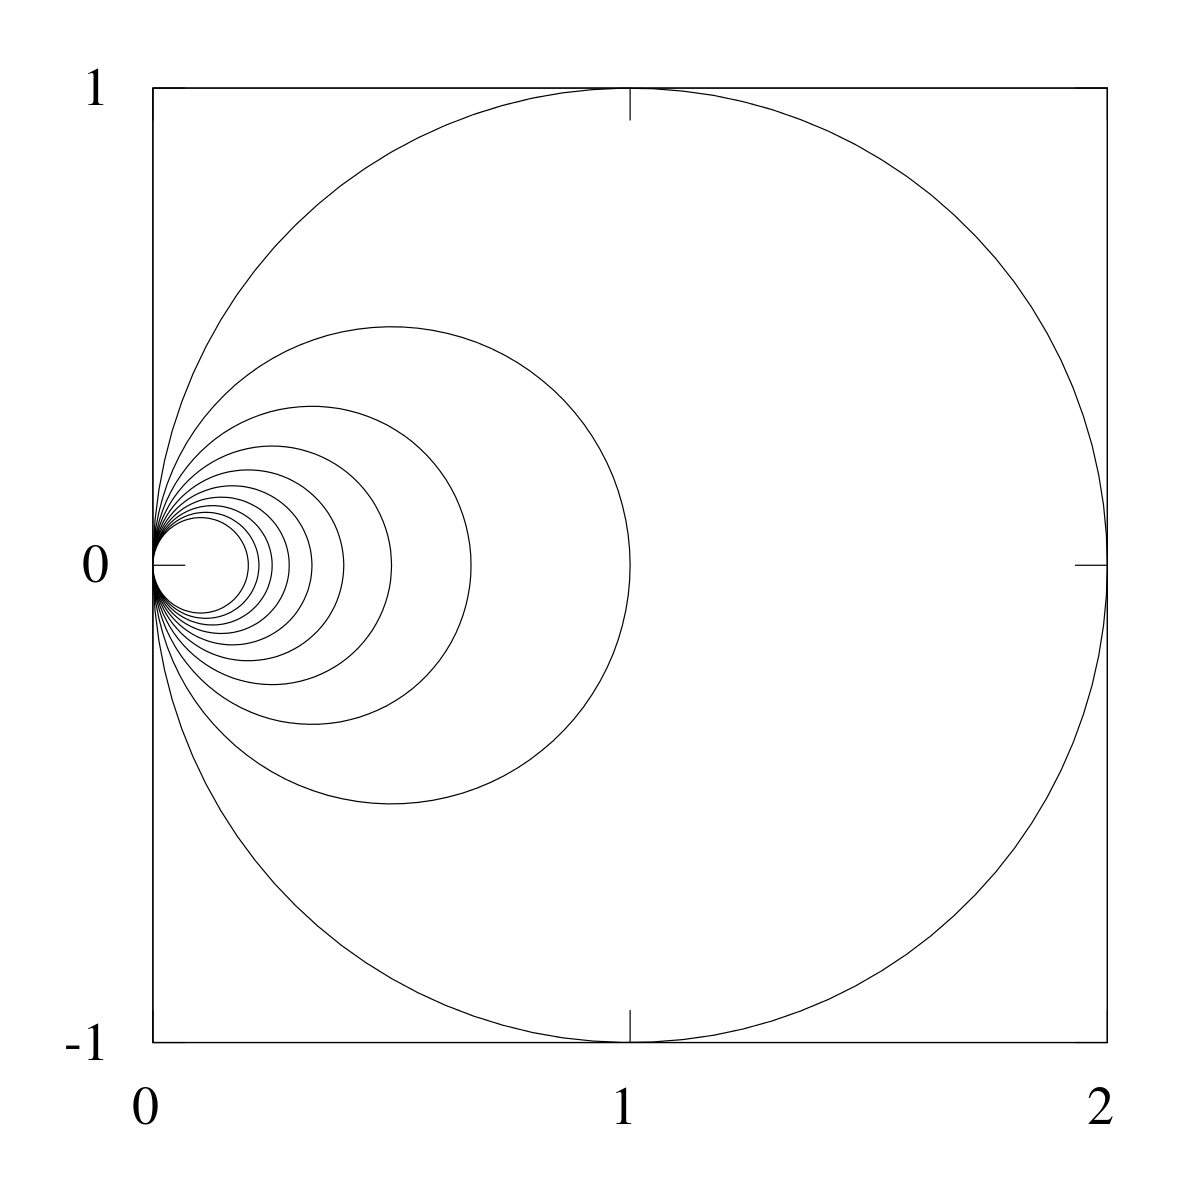
\includegraphics[width=10cm]{images/m4_earring.png}
\caption{\small{The Hawaiian Earring}}
\label{img:m4_hawaiianearring}
\end{figure}
This is not semi-locally simply connected, since all neighborhoods of $(0, 0)$ contain one of the circles centered at $(\frac{1}{n}, 0)$ with radius $\frac{1}{n}$, so there is a non-contractible loop in all neighborhoods of $(0, 0).$

Note the difference between semi-locally simply connected and locally simply connected. A space $X$ is locally simply connected if for all $p\in X$, for all neighborhoods $U$ of $x,$ there exists a neighborhood $V\subset U$ of $x$ which is simply connected. That means all loops in $V$ are contractible in $V,$ not in $X$. In the definition of semi-locally simply connected, loops in $U$ must be contractible to a single point, but that contraction need not take place in $U.$ There are sets that are semi-locally simply connected but not locally simply connected. For instance, consider the subset of $\mathbb{R}^3$ that consists of the Hawaiian Earring on the $xy$-plane, the point $(0, 0, 1)$, and all line segments between the point $(0, 0, 1)$ and the points on the Hawaiian Earring. 

This space is semi-locally simply connected but not locally simply connected, since every loop in the space can be continuously deformed to the point $(0, 0, 1)$, but in all neighborhoods of $(0, 0, 0)$ contain in the ball with radius $\frac{1}{2}$ around $(0, 0, 0),$ there is a loop in the neighborhood that cannot be deformed within the neighborhood, since it can only be deformed to the point $(0, 0, 1).$

\subsection{Locally Path Connected}
A space $X$ is locally path connected if, for all $x\in X$, for all neighborhoods $U$ of $x$, there exists a neighborhood $V\subset U$ of $x$.
\subsubsection{Examples and nonexamples}
Note that the Hawaiian Earring is locally path connected and connected, but not semi-locally simply connected. The space $[-2, -1]\cup [1, 2]$ is locally path connected and semi-locally simply connected, but not connected. The comb space, which is $\{(x, 0) |x\in [0, 1]\}\cup \cup_{n\in \mathbb{N}} \{(\frac{1}{n}, y)|y\in [0, 1]\},$ is connected and semi-locally simply connected, but not locally path connected. Near $(0, \frac{1}{2})$, some neighborhoods contain no smaller, path connected neighborhoods.
\begin{figure}[H]
\centering
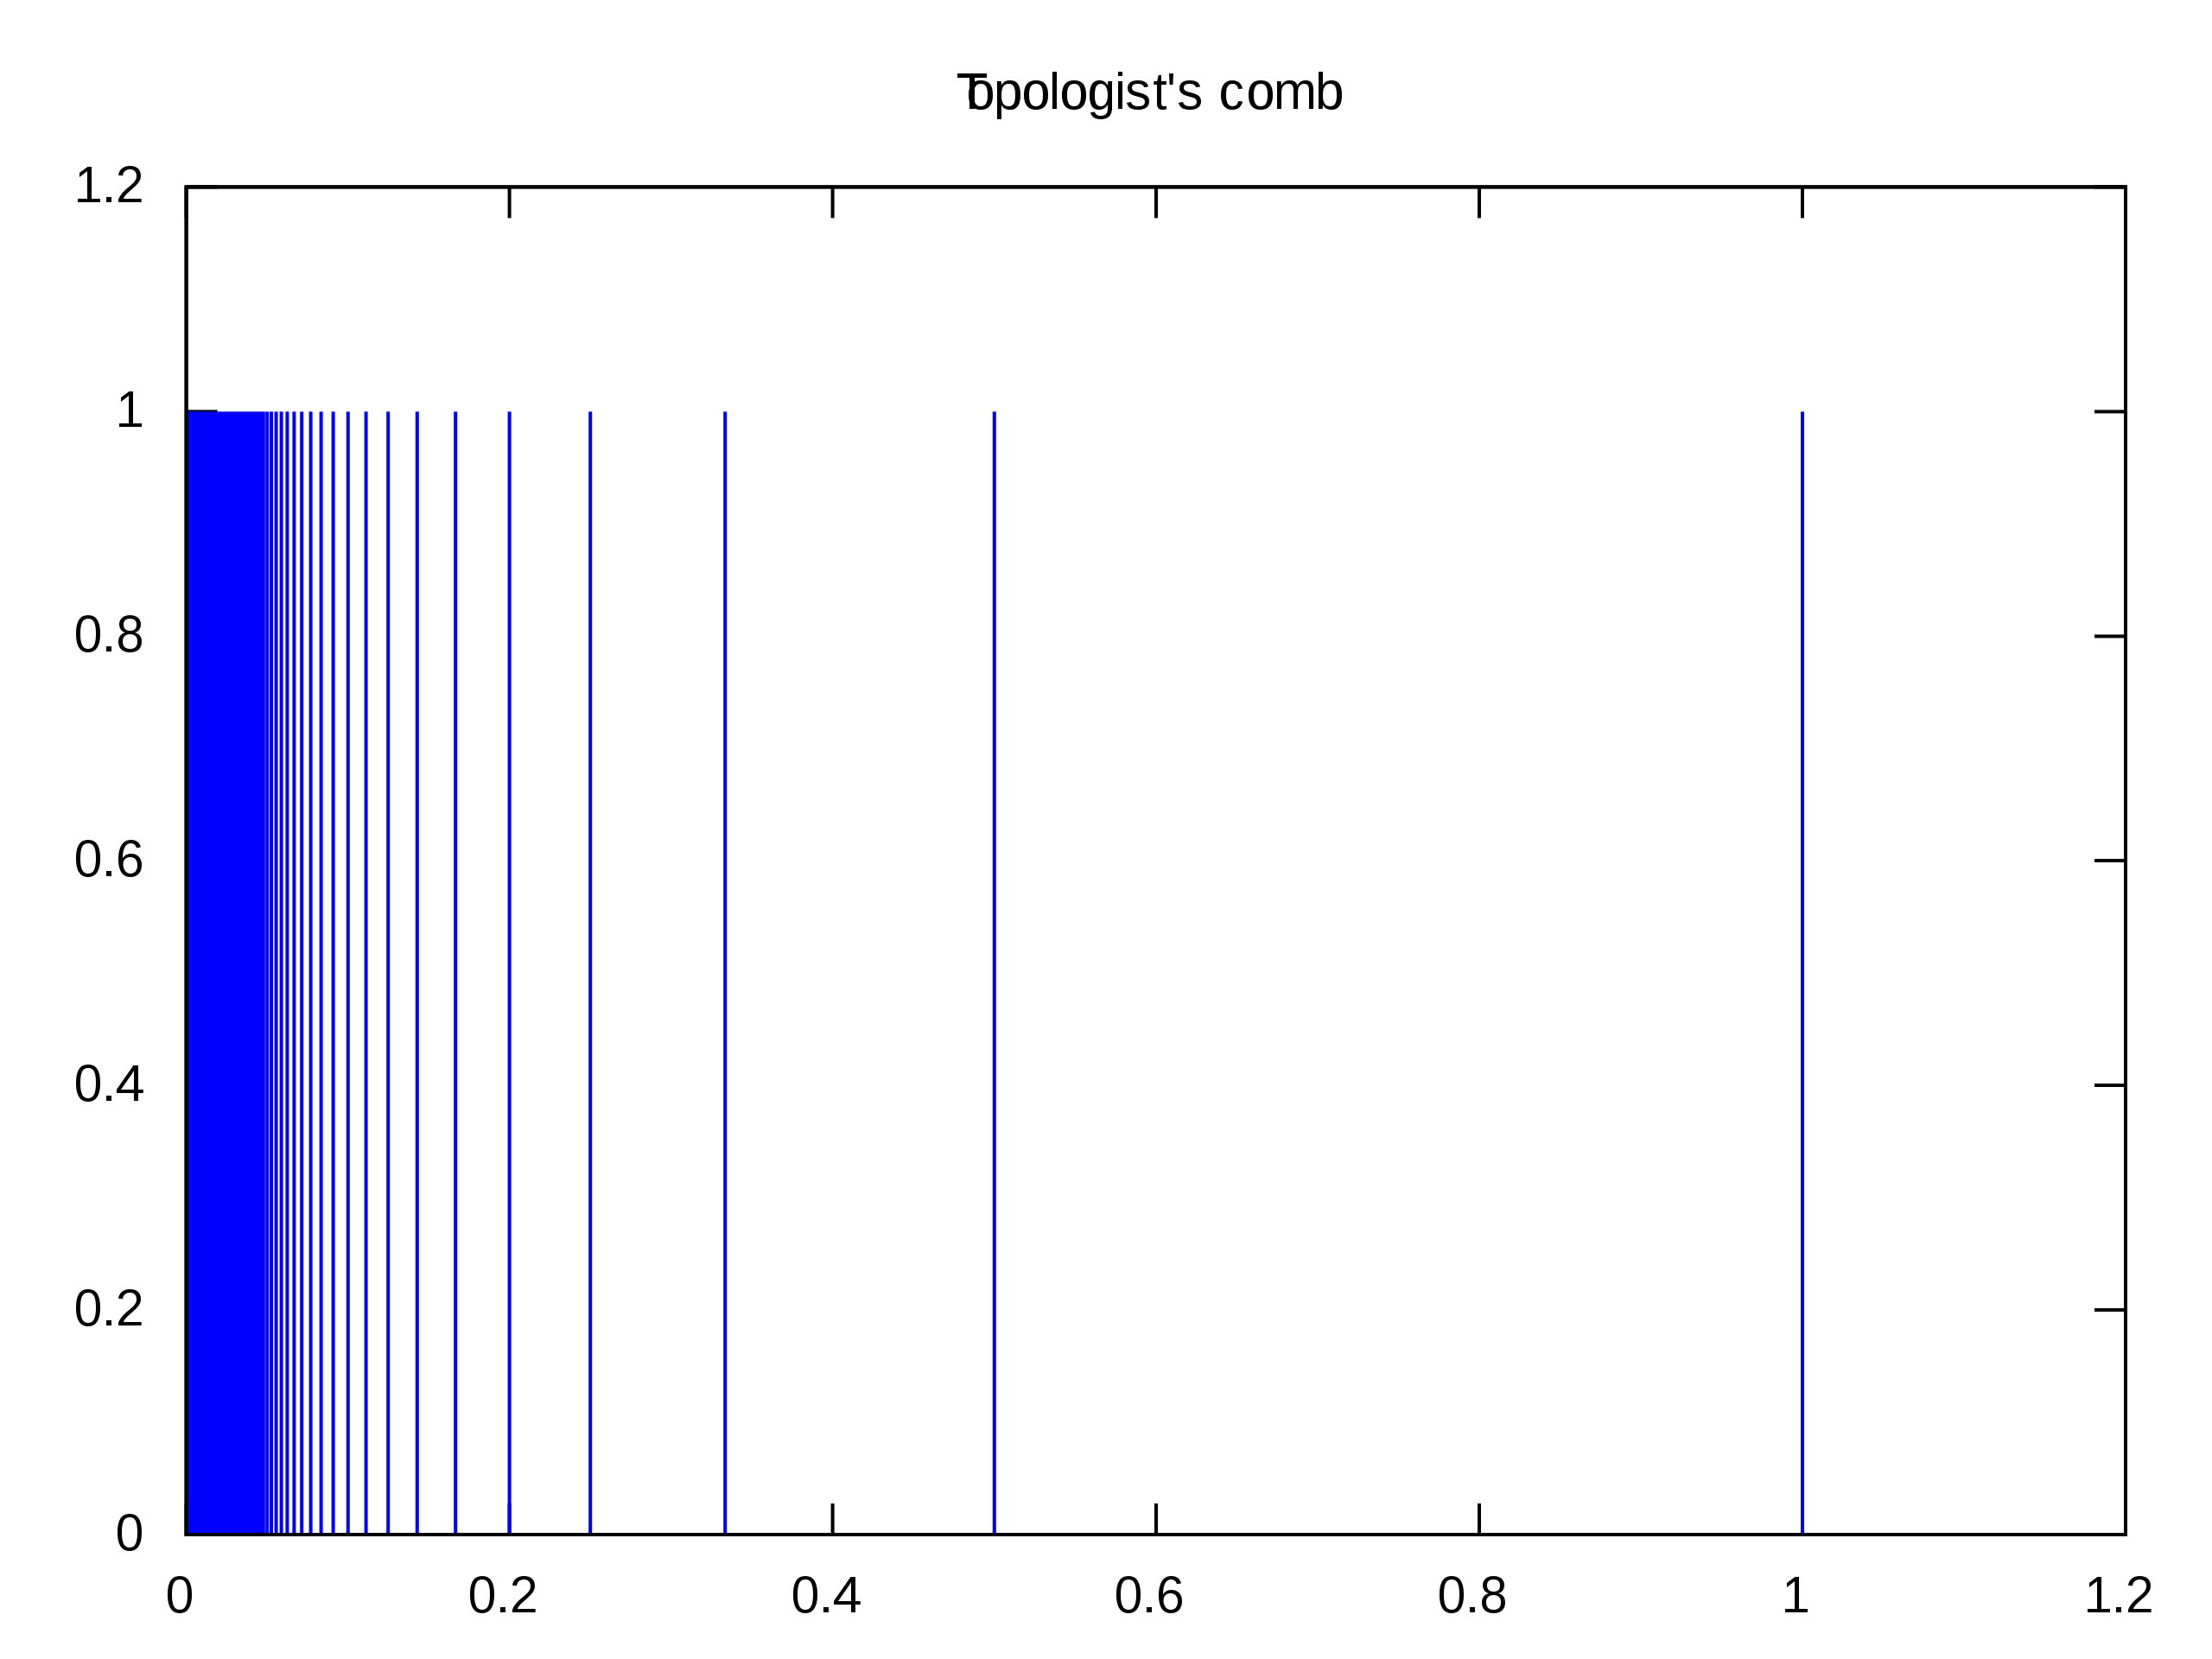
\includegraphics[width=10cm]{images/m4_comb.png}
\caption{\small{Comb space}}
\label{img:m4_combspace}
\end{figure}
So, none of the three assumptions for a universal covering are redundant.

\section{Deck transformations}
\begin{keyterm}{Deck transformations}
Suppose $p_1: \tilde{X}_1 \to X$ and $p_2:\tilde{X}_2 \to X$ are two covering spaces. A homomorphism between covering spaces is denoted as $\alpha: \tilde{X}_1 \to \tilde{X}_2$ where $p_1 = p_2 \circ f$ (where $f$ could be an isomorphism between the covering spaces). Particularly, if $f$ is an isomorphism between a covering space and itself, we call that a \newword{deck transformation} as it simply serves to permute the fibers of the covering map.

The set of deck transformations of a covering space is a group under the binary operation of composition.
\end{keyterm}

\begin{theorem}
\textbf{Action of $\pi_1$ on a universal cover}\\ 
The following are equivalent:\\
(a) $p: X \to Y$ is a regular covering space\\
(b) $p_{*}(\pi_{1}(X))$ is normal in $\pi_{1}(Y)$\\
(c) $D(X) = \pi_{1}(Y)/H$ where $H = p_{*}(\pi_{1}(X))$ is the \emph{deck group}
\end{theorem}

We state importantly that for a covering space $p: X \to Y$, it always follows that $p_{*}(\pi_{1}(X)) < \pi_{1}(Y)$. The extra condition of $p$ being a \emph{regular} covering specifies that $p_{*}(\pi_{1}(X))$ is in fact a \emph{normal} subgroup of $\pi_{1}(Y)$.

\textbf{Restatement of the uniformization theorem}\\
Let $W$ be a simply connected Riemann surface. Then if \cite{uniformization_theorem_pf_marshall}
\begin{enumerate}
    \item If Green's function exists on $W$, biholomorphic map to $\DD$
    \item If $W$ is compact, biholomorphic map to $\hat{\CC}$
    \item If Green's function does not exist and $W$ is not compact, biholomorphic map to $\CC$ 
\end{enumerate}

\textbf{Genus relationship}
If genus of a Riemann surface is equal to 
\begin{enumerate}
    \item 0 $\Rightarrow$ universal cover is $\hat{\CC}$
    \item 1 $\Rightarrow$ universal cover is $\CC$
    \item else $\Rightarrow$ universal cover is $\DD$
\end{enumerate}

\mainpoint{Every connected Riemann surface can be viewed as the quotient of its simply connected universal cover (one of the three in the \textit{Genus relationship} by a discrete group of automorphisms (\textit{deck transformations})}

% MEETING 5
\lecture{5}{Basics of Complex Analysis}{May 21-22}{Drimik Roy}
\setcounter{section}{0}
\section{Key points from meeting}
\begin{enumerate}
    \item If $p: X \to Y$ is a \emph{regular} covering space, then loops in $Y$ lift to loops in $X$. 
    \item A key point of this research is to identify if flat connections on Riemann surfaces have any relationship with dessin d'enfants on Riemann surfaces.
    \item $\chi(\Sigma_{g,n}) = 2-(2g+n)$ where $g$ is the genus and $n$ is the number of punctures on the Riemann surface $\Sigma_{g,n}$.
\end{enumerate}

\section{Introductory results from complex analysis}
These notes on Complex Analysis are inspired from Steven J. Miller's course. Visit \href{}{here} for more

Let $f: \RR \to \RR$ be differentiable.
\begin{center}
\begin{tabular}{|m{8cm}|m{3cm}|m{4cm}|}
    \hline
    Questions & Real differentiable & Complex differentiable \\
    \hline
    With $f$ being differentiable, then $f$ is infinitely differentiable & NO & YES \\
    \hline
    Suppose $f$ is infinitely differentiable. Then $f$ is given by its Taylor series expansion in a \nghd of a point & NO & YES \\
    \hline
    $f$ can be defined everywhere and be bounded and not be constant & YES & NO \\
    \hline
    A line integral of $f$ over a closed curve is zero & NO & YES \\
    \hline
\end{tabular}
\end{center}

The third statement arises by the statement of \textbf{Liouville's theorem}, which states that every bounded \emph{entire function} is constant. This is proved in \textbf{TODO}. Furthermore, if $f$ is differentiable at $z_0 \in \CC$, then $f$ is said to be analytic on a \nghd around $z_0$.

\section{Notes on Chapter 1: From Complex Analysis to Riemann Surfaces} 
Notes mainly from "Riemann surfaces and Algebraic Curves" \cite{riemann_surfaces_algebraic_curves}.

\begin{keyterm}{Cauchy-Riemann Equations}
Let $f:\CC \to \CC$ be defined as $f(z)= u(x,y) + iv(x,y)$. The \newword{Cauchy-Riemann equations} are defined as follows:
\begin{align*}
    \frac{\partial u}{\partial x} &= \frac{\partial v}{\partial y} \\
    \frac{\partial u}{\partial y} &= -\frac{\partial v}{\partial x}
\end{align*}
\mainpoint{$f$ is complex differentiable $\Leftrightarrow$ $f$ satisfies the Cauchy Riemann equations.}
\end{keyterm}


\begin{theorem}
\newword{Green's theorem} Let $\Omega$ be a closed boundary region where $\partial \Omega$ is the boundary which has no holes and "nice". Define function ${F}(x,y) = (P(x,y), Q(x,y))$ with the property that 

\begin{align*}
\begin{split}
    \oint_{\partial \Omega} \vec{F}(x,y) d\vec{s}
    &= \oint_{\partial \Omega} P dx + Q dy \\
    &= \iint_{\Omega} (\frac{\partial Q}{\partial x} - \frac{\partial P}{\partial y}) dx dy
\end{split}
\end{align*}
\end{theorem}

\begin{theorem}
\newword{Open mapping theorem} A non-constant holomorphic function $f$ is an open map. 
\end{theorem}

\subsection{Integration}
Let $f$ be a holomorphic function and $\gamma:[a,b] \to \CC$ be a path. Then $\int_{\gamma} f(z) dz = \int_a^b f(\gamma(t))\gamma'(t) dt$.

\begin{claim}\label{exc:blue_book_1.2.1}
\underline{Exercise 1.2.1}
Show that, for any integer $n \ne -1$, the integral $\int_{\gamma} z^n dz = 0$ where $\gamma$ is a circle of radius $r$ centered at zero.
\end{claim}
\begin{proof}
Parametrize $\gamma$ as $\gamma(t) = re^{2\pi i t}$ for $t \in [0,1]$.
\begin{align*}
\begin{split}
    \int_{\gamma} z^n dz
    &= \int_0^1 (re^{2{\pi}it})^n (2{\pi}ire^{2{\pi}it}) dt \\
    &= 2{\pi}ir^{n+1} \int_0^1 e^{i(2{\pi}it(n+1))} dt \\
    &= 2{\pi}ir^{n+1} \int_0^1 cos(2{\pi}t(n+1)) + isin(2{\pi}t(n+1)) dt \\
    &=
\begin{cases}
    2{\pi}i & n = -1 \\
    0 & otherwise
\end{cases}
\end{split}
\end{align*}
\end{proof}

For $f: \CC \to \CC$ to be complex differentiable, many was for $h \rightarrow 0$ in the definition of differentiability as $\CC \isom \RR^2$. Thus, greater structure forced on complex differentiable functions compared to real.

Whenever $f'$ does not vanish, multiple local inverse functions exist and we say the inverse of $f$ is said to be a multivalued function. The local inverses create a global function on a space that locally $\isom \CC$ but globally may be very different. These are the \emph{Riemann surfaces}.

\begin{theorem}\label{thm:holomorphic_ftn_homotopic_implies_same_integral}
Suppose $\gamma, \mu: [a,b] \to U \subseteq \CC$ are homotopic. Then for any holomorphic function $f$ on $U$, we have 
\begin{equation*}
    \int_{\gamma} f(z) dz = \int_{\mu} f(z) dz
\end{equation*}
\end{theorem}

\begin{corollary}
If $U \subseteq \CC$ is a simple connected region and $f$ holomorphic function on $U$. For any closed path i.e. loop in $U$, we have that $\oint_{\gamma} f(z) dz = 0$. 
\end{corollary}
\begin{proof}
$\gamma$ homotopic to a point since $U$ simply connected and apply Theorem \ref{thm:holomorphic_ftn_homotopic_implies_same_integral}.
\end{proof}

\begin{claim}\label{exc:blue_book_1.2.2}
\underline{Exercise 1.2.2}
Let $U \subseteq \CC$ be an open set and $f$ a holomorphic function on $U\setminus \{z_0\}$. For $j=1,2,$ let $\gamma_j$ be a path parameterizing a circle centered at $z_0$ of radius $r_j$, oriented counterclockwise and completely contained in $U$. Show that 
\begin{equation*}
    \oint_{\gamma_1} f(z) dz = \oint_{\gamma_2} f(z) dz
\end{equation*}
\end{claim}
\begin{proof}
Since the two loops $\gamma_1$ and $\gamma_2$ are oriented in the same direction, they are homotopic. Apply Theorem \ref{thm:holomorphic_ftn_homotopic_implies_same_integral}.
\end{proof}

\begin{claim}
Let $\gamma$ be a circle of radius centered at 0. Evaluate $\int_{\gamma} 1/z dz$.
\end{claim}
\begin{proof}
Parameterize $\gamma$ as $\gamma(t) = re^{2{\pi}it}$.
\begin{equation*}
    \int_{\gamma} \frac{1}{z} dz 
    = \int_0^1 \frac{1}{re^{2{\pi}it}} 2{\pi}ire^{2{\pi}it} dt
    = \int_0^1 2{\pi}i dt 
    = 2{\pi}i
\end{equation*}
\end{proof}

\subsection{Cauchy's Integral Formula}
\begin{theorem}
\textbf{Cauchy's Integral Formula} Let $U \subseteq \CC$ be an open set. Define $D$ as a closed disk within $U$ where $\gamma$ is a circle defined as the boundary of $D$. Let $f$ be a holomorphic function on $D$. Then we have that for any $z$ in the \emph{interior} of $D$. 
\begin{equation*}
    f(a) = \frac{1}{2{\pi}i} \oint_{\gamma} \frac{f(z)}{z-a} dz
\end{equation*}
\end{theorem}
Why we should believe it: From Theorem \ref{thm:holomorphic_ftn_homotopic_implies_same_integral}, $\gamma$ bounds a small disk around $a$ with the same integral value and by Exercise \ref{exc:blue_book_1.2.2}, can let radius this small disk shrink to 0 without changing value of integral. Then $f(z)$ restricted to $\gamma$ tends to the value $f(a)$ while the path integral of $\frac{1}{z-a}$ is $2{\pi}i$ by the previous claim.
\begin{proof}

\end{proof}

The key fact is that $f$ is completely determined within $D$ just by knowing the values of $f$ along $\gamma$, the boundary of $D$. 

\textbf{Major consequence of Cauchy's integral formula}
\begin{enumerate}
    \item Holomorphic functions on an open set are infinitely differentiable
    \item Holomorphic functions $\Leftrightarrow$ analytic functions
\end{enumerate}

TODO:
\begin{enumerate}
    \item look into meromorphic functions with prescribed poles
    \item Notes from Ch1, Ch2 on Riemann surfaces and algebraic curves book
\end{enumerate}

\section{Meromorphic functions}

% MEETING 6
\lecture{6}{Monodromy and clarifications on covering spaces}{May 24}{Drimik Roy}
\setcounter{section}{0}

\section{Monodromy}
Let $p: X \to Y$ be a covering space and let $E \subseteq X$ where $E = p^{-1}(y_0)$ i.e. the fibers of $y_0 \in Y$.

Let $\gamma \in \pi_{1}(Y,y_0)$, then $\gamma$ induces a bijection $g: E \to E$ because 
\begin{enumerate}
    \item $\gamma$ is a closed oriented curve with $p^{-1}(\gamma)$ consists of deg $p$ many oriented curves.
    \item $\gamma$ from $y_0$ to $y_0$ as it is a loop so each $\phi \in p^{-1}(\gamma)$ is from $x_0 \in E$ to $x_1 \in E$.
    \item $g$ is bijective because $\gamma$ is invertible in $\pi_{1}(Y,y_0)$.
\end{enumerate}

We note that $\gamma \mapsto g$ is a group homomorphism from $\pi_{1}(Y,y_0)$ to the group of bijections on $E$ where the product of paths in $\pi_{1}(Y,y_0)$ is associated with teh composition of the bijections on $E$. 

\mainpoint{The image of this group homomorphism in $E$ is the \newword{monodromy group} of the covering map.}

Note then that \underline{$\pi_{1}(Y,y_0)$ is acting on $E$}.

\section{Coverings}
We note that \underline{unramified coverings = coverings}. 

\begin{keyterm}{nowhere dense set}
A \newword{nowhere dense set} $E$ is a set such that the closure of $E$ contains no nonempty open intervals. For example $E = \{1/n | n \in \NN\}$ is a nowhere dense set as $\Bar{E} = \{1/n | n \in \NN\} \union \{0\}$ which has no nonempty open intervals contained in $\Bar{E}$.
\end{keyterm}

\begin{keyterm}{branch covering}
$p: X \to Y$ is a \newword{branch covering} if it is "almost" a covering map. That is, $p$ is a covering map everywhere except for a nowhere dense set which is known as the \newword{branch set}. 
\end{keyterm}

If $p: X \to Y$ is a ramified covering, then $p$ is a continuous mapping and all points of $Y$ \emph{except countably many} have the same number of pre-images. We say that for these countably many elements of $Y$, each $y_0 \in Y$ with this property is a \newword{critical value} or a \newword{ramification point} with a certain \emph{multiplicity} to account for the degree of $p$. 

In addition, let $p: X \to Y$ be a covering space. Then deg $p = [\pi_{1}(Y) : \pi_{1}(X)]$ i.e. the index of the subgroup $pi_{1}(X)$ of $\pi_{1}(Y)$. Note that we are assuming the two spaces $X,Y$ are path connected to identify a single fundamental group for the entire spaces.

If $y \ne \infty$ is a critical value of $p$ then $p(x) = y$ has $< n$ solutions where deg $p = n$ at non-critical values. If $x_0 \in X$ is a solution to $p(x) = y$, then $p'(x_0) = 0$. In other words, a critical value of $p$ is a value of $p$ such that the it is a zero of the derivative. We denote $x_0$ as a \newword{critical point} of $p$ associated $y_0$. The \newword{multiplicity} of $x_0$ is equal to $d \geq 2$ where $p'(x_0) = 0, p''(x_0) = 0,...p^{(d)}(x_0) \ne 0$.

TODO
\begin{enumerate}
    \item diff between orbifold covering, branch cover, covering space
    \item why pre-image of every pair of points in base space has always the same number of points in the covering space
    \item pg 4 of Tech muler only cnn 2 points at a time, not 3. Why??
    \item elliptic integrals
\end{enumerate}

% MEETING 7
\lecture{7}{Belyi Functions and Dessins}{June 3}{Drimik Roy}
\setcounter{section}{0}

The study of Belyi functions is the theory of \newword{dessin d' enfants}. The important claim is that for a Riemann surface $X$, we say that $X$ admits a Belyi function i.e. embeds a dessin iff $X$ is defined over the field $\Bar{\QQ}$ of algebraic numbers. 

We will only consider connected graphs where loops and multiple edges are allowed. All maps will be oriented.

The sections before \nameref{sec:m8_intro_galois_theory} are inspired from \cite{belyi_functions_examples_zvonkin}.

\section{Maps and Hypermaps}
\begin{keyterm}{Map}
A \newword{map} is a graph embedded in a \emph{compact oriented} two-dimensional manifold s.t.
\begin{itemize}
    \item the edges don't intersect
    \item the complement of the graph in the surface is a disjoint union of regions homeomorphic to the open disks
\end{itemize}
These regions are the \newword{faces} of the map and the \newword{genus} of the map is the genus of the underlying surface.
\end{keyterm}
\begin{keyterm}{Hypermap}
A \newword{hypermap} is a bicolored map.
\end{keyterm}

We can obtain a hypermap $H$ from a map $M$ by inserting a white vertex in between every edge between two vertices. Hence, every white vertex will have degree $2$ and we say by convention that each edge between a black and white vertex is instead a \emph{half-edge}. 

Hence, we can rewrite the Euler characteristic of $H$ with $n$ half-edges as 
\begin{equation*}
    \chi(H) = 2-2g = B + W + F - n
\end{equation*}

since for each newly added white vertex we split an edge into two half-edges.

\subsection{Encoding hypermaps by triples of permutations}
The key idea is that hypermaps can be constructed from a triple of permutations. We use the fact that the surface on which the hypermap is embedded is \emph{oriented}. Every half-edge has a left/right bank and there is a positive/negative orientation around every vertex (positive being counterclockwise). 

Let $H$ be a hypermap with $n$ half-edges and label each half-edge from $1$ to $n$ and place them on the left bank of the half-edge from the black to the white vertex. The triple of permutations $(\sigma, \alpha, \phi)$ on the set of $n$ labels associated to $H$ is:
\begin{itemize}
    \item A cycle of $\sigma$ contains the labels of the half-edges incident to a particular black vertex taken in the positive i.e. counterclockwise direction. Note then there are as many cycles as there are black vertices and the left of each cycle corresponds to the number of half-edges incident to the black vertex in question. \item Similarly, we have cycles of $\alpha$ for white vertices.
    \item A cycle of $\phi$ contains labels placed inside a face taken in the positive direction around center of face.
\end{itemize}

\begin{figure}[H]
\centering
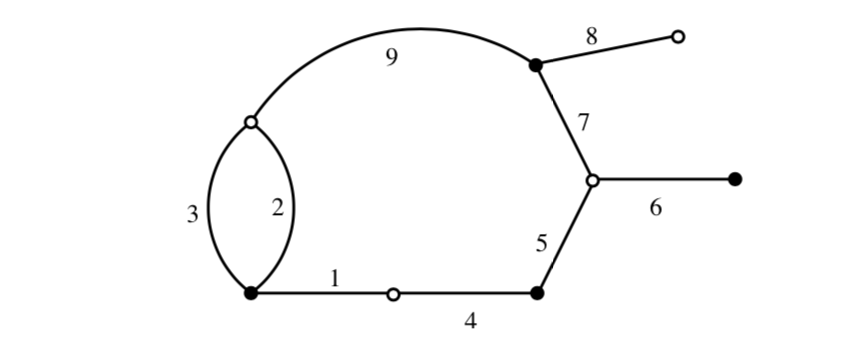
\includegraphics[width=10cm]{images/m8_triple_permutations_hypermap.png}
\caption{\small{Example of hypermap labelling}}
\label{img:m8_triple_permutations_hypermap}
\end{figure}

Based on Figure \ref{img:m8_triple_permutations_hypermap}, we have the following permutations:
\begin{align*}
    \sigma &= (123)(45)(6)(789)\\
    \alpha &= (293)(14)(567)(8)\\
    \phi &= (159)(2)(43876)\\
\end{align*}
Note that $(43876)$ appears to be in the negative direction but for the outer face, take the perspective as you are in the "center of the manifold" and looking out. Hence, we arrive that this cycle is in fact in the positive direction around the "center of the outer face".

\mainpoint{
For any hypermap $H$ with $n$ half-edges, we can see the aforementioned triple of permutations $(\sigma, \alpha, \phi)$ has the property that $\sigma\alpha\phi = (1)$. So, we only need 2 of the three permutations to encode a hypermap.
}

In the converse direction, for every triple of permutations such that 
\begin{itemize}
    \item the permutation group $G=\langle \sigma,\alpha,\phi \rangle$ is transitive
    \item $\sigma\alpha\phi = (1)$ 
\end{itemize}
there corresponds a hypermap. The need for the transitive action guarantees that the graph is connected.

We call $G=\langle \sigma,\alpha,\phi \rangle$ the \newword{cartographic group} associated with hypermap $H$.

\subsection{Transitive and Faithful group actions}
Let $G$ be a group and $X$ be a set. The action of $G$ on $X$ is \newword{transitive} if $X$ is non-empty and $\forall x,y \in X$, $\exists g \in G$ such that $g \cdot x = y$. That is, there exists only one orbit.

The action of $G$ on $X$ is \newword{faithful} if for each $g \in G$ s.t. $g \ne e$, we have that $\exists x \in X$ such that $g \cdot x \ne x$. As a contrapositive, there exists no $g \in G$ except for $g = e$ such that $g \cdot x = x$, $\forall x \in X$.

\section{Belyi functions: planar case}
\begin{keyterm}{Belyi function}
Let $H$ be a planar hypermap with $n$ half-edges. A rational function $f$ of degree $n$ is a \newword{Belyi function} associated with $H$ if $H$ can be embedded into the Riemann complex sphere $\hat{\CC}$ where
\begin{enumerate}
    \item Black vertices of $H$ correspond to roots of $f(x)=0$ and multiplicity of root $=$ degree of vertex
    \item White vertices of $H$ correspond to roots of $f(x)-1=0$ and multiplicity of root $=$ degree of vertex
    \item Hypermap $H$ is pre-image of $[0,1]$ i.e. $H = f^{-1}([0,1]$.
    \item Inside each face of $H$ exists a \emph{single} pole of $f$ or root of equation $f(x) = \infty$ where multiplicity of pole = degree of face. The pole is called the \newword{center} of face.
    \item No other critical values of $f$ other than $0,1,\infty$.
\end{enumerate}
A \newword{critical point} of $f$ is a root of the derivative and a \newword{critical value} of $f$ is $f$ at a critical point.

Note that for any $f$ with three critical values, we can apply any linear fractional transformation and move these critical values to $0,1,\infty$.
\end{keyterm}

\begin{theorem}
For every hypermap $H$, there exists a corresponding Belyi function $f$. The function is unique up to a linear fractional transformation.
\end{theorem}

\noindent\fbox{%
    \parbox{\textwidth}{%
        \textbf{Important question:} Given a hypermap $H$, how to construct the corresponding Belyi function?
    }
}

\section{Belyi functions: non-planar case} 
This section is inspired from \cite{belyi_functions_examples_zvonkin}.

For $g=0$, we can construct maps that are planes which would have graphs that are planar. Now, for $g \geq 1$, there are infinitely many non-isomorphic Riemann surfaces. For these cases, we have to talk about a \emph{Belyi pair} rather than a Belyi function on its own.

\begin{theorem}
\textbf{Belyi's theorem}

Let $X$ be a Riemann surface. The following statements are identical in meaning.
\begin{enumerate}
    \item $X$ admits a model over the field of algebraic numbers $\Bar{\QQ}$ iff there exists an $f: X \to \CC$ unramified outside of $\{0,1,\infty\}$.
    \item A nonsingular algebraic curve can be defined over $\Bar{\QQ}$ iff as a Riemann surface, it admits a holomorphic function onto the Riemann sphere that is ramified at only three points.
\end{enumerate}
\end{theorem}

\begin{keyterm}{Belyi pair} 
Let $X$ be a Riemann surface and $f: X \to \hat{\CC}$ be a meromoprhic function on $X$ that is unramified outside of $\{0,1,\infty\}$. Then $(X,f)$ is a Belyi pair.
\end{keyterm}

\section{Galois Theory}
\label{sec:m8_intro_galois_theory}
\subsection{Motivation}
The motivation for Galois theory was constructed by identifying that the roots of the polynomial $f$ over the field $F$ have a sense of symmetry to them that can be revealed by a group acting on them (Galois group of $f$). By studying the permutation groups of the polynomial roots, Galois found a necessary and sufficient condition to find the roots of a $nth$ degree polynomial based on some algebraic combination $+,\cdot,\sqrt{}$ of the coefficients.

When the problem is stated from the Field theory to Group theory, Galois theory serves as the dictionary to communicate this concept. 

\subsection{Galois Group}
Let $F$ be a field where $E \subseteq F$. Suppose that $E$ is a field with the properties of $F$ restricted to $E$. Then we say that $F$ ($E)$ is a \newword{field extension} (\newword{subfield}) of $E$ ($F$). An automorphism of $F/E$ fixes $E$ pointwise. The set of automorphisms of $F/E$ under the binary operation of function composition forms a group. This group is denoted as $Aut(F/E)$. 

\begin{keyterm}{Algebraic field extension}
We say that $F/E$ is a \newword{algebraic field extension} if every element $\alpha \in F$ is a root of some nonzero polynomial with coefficients in $E$. 
\end{keyterm}

\begin{keyterm}{Normal extension}
An algebraic field extension $F$ of $E$ where every irreducible polynomial over $E$ has no roots in $F$ or has linear factors in $F$.
\end{keyterm}
\begin{keyterm}{Separable extension}
An algebraic field extension of $F$ of $E$ s.t. $\forall \alpha \in F$, the \emph{minimum polynomial} of $\alpha$ in $E$ is separable i.e. has \emph{distinct} roots in the algebraic closure of $E$.
\end{keyterm}

Now, we say that $F/E$ is a \newword{Galois extension} if it is an algebraic field extension that is both normal and separable. If $F/E$ is a Galois extension, then $Aut(F/E)$ is the \newword{Galois group of $F$ over $E$}.

\begin{claim}
Let $f$ be a polynomial defined over $F$. Suppose $K$ is the splitting field of $F$ formed by one by one \newword{adjoining} the $n$ roots of $f$ to $F$ and creating the following tower of fields $F \subseteq F_1 \subseteq F_2 \subseteq ... \subseteq F_n := K$. 

Then by noticing that $K$ is a field extension of $F$, it is easy to see that the Galois group of $K$ over $F$ $Aut(K/F)$ are simply permutations of the $n$ roots of $f$ as the base field $F$ are fixed in the automorphisms. Hence, the Galois group is in fact isomorphic to some subgroup of $S_n$. 

Through this property, we can see that the action of the Galois group is essentially associated some permutation of the roots of $f$.
\end{claim}

\subsection{Rationals $\QQ$}
We note that the algebraic closure of $\QQ$ i.e. the smallest algebraic extension of $\QQ$ that is algebraically closed is $\Bar{QQ}$ or simply the \emph{algebraic numbers}.

\begin{claim}
$\QQ$ is a \newword{perfect} field
\end{claim}
\begin{proof}
Since every irreducible polynomial of degree $n$ over $\QQ$ factors into $n$ distinct roots over $\Bar{\QQ}$ by definition of $\Bar{\QQ}$, we have that $\QQ$ is a perfect field.
\end{proof}

\begin{theorem}
If $K$ is a perfect field, then the separable closure of $K$ is the algebraic closure of $K$.
\end{theorem}
\begin{proof}
Every algebraic extension of $K$ is separable by definition of $K$ being a perfect field. Since $K^{alg}$ is the "largest" algebraic extension of $K$, follows that the separable closure of $K$ is $K^{alg}$.
\end{proof}

\mainpoint{Since $\QQ$ is a perfect field, we have that $\QQ^{sep} = \QQ^{alg} = \Bar{\QQ}$.}

\begin{theorem}
If the algebraic closure of $K$ is a Galois extension, then $K$ is a perfect field.
\end{theorem}

\subsection{Absolute Galois Groups}
We have now identified that the Galois groups are in some sort permutations over the roots of polynomials. 

Let $K$ be a field and let $K^{sep}$ be the separable closure of $K$.
The absolute Galois group of $K$ is defined as the Galois group of $K^{sep}$ over $K$. 

\underline{Why is the Gal$(\Bar{\QQ} \backslash \QQ)$ so important?}
\href{https://math.stackexchange.com/questions/805088/why-there-is-much-interest-in-the-study-of-operatornamegal-left-overline-m/806525}{Visit this discussion}


\section{History of \textit{Esquisse d'un programme}}
This section is inspired from \cite{actions_of_abs_group_lizhen}.

This proposal was created for the purposes of extending and generalizing Galois theory. One of Grothendieck's inspirations was to study the absolute Galois group of the rationals $\Gamma_{\QQ} := $ Gal$(\hat{\QQ} \backslash \QQ)$. His idea was that if we can cause $\Gamma_{\QQ}$ to act on geometric objects (because in some sense the automorphisms on these objects were "tractable"), then ideally we could have some injective map between $\Gamma_{\QQ}$ and automorphisms on the geometric objects.

\begin{keyterm}{Dessin d'enfant}
A bipartite graph $G$ on a compact oriented surface $S$ that is the pre-image of the unit interval $[0,1]$ by a holomorphic function to $\hat{\CC}$ that is ramified at $0,1,\infty$ where the following properties are held 
\begin{enumerate}
    \item $S \setminus G$ is a disjoint collection of open sets (homeomorphic to open disk)
    \item Vertices of the fiber of $0$ and $1$ are black and white, respectively, so no every edge connects vertices of different colors
\end{enumerate}
\end{keyterm}

As a recap, we know that by Belyi's theorem states that a nonsingular curve can be defined over $\hat{\QQ}$ iff when the curve is viewed as a Riemann surface, there exists a holomorphic function to $\hat{\CC}$ that is ramified only at 3 points. Hence, we see there is a direct relationship between the Dessins and Belyi's theorem. The function in question is \emph{Belyi's function} and Dessins are simply then the study of these Belyi functions.

A key idea was to study the correspondence of the action of the absolute Galois group of the coefficients in $\Bar{\QQ}$ for these polynomials (nonsingular algebraic curves) and the action on the dessins as the combinatorial objects. It was proved that this action is indeed \emph{faithful}, which would mean that any non-identity element of $\Gamma_{\QQ}$ sends at least one dessin to a non-isomorphic dessin or simply that every element of the Galois group of the algebraic numbers determines a different permutation of the set of dessins. This finding serves as the combinatorial foundation to understanding $\Gamma_{\QQ}$.

% LECTURE 8
\lecture{8}{Hypergeometric Functions, Fuchsian ODEs}{June 25}{Drimik Roy}
\setcounter{section}{0}
Now we shall view the relationship of Dessin d'enfants and solutions to Fuchsian differential equations as the open-ended research question for the REU. The hypergeometric differential equation acts as a guide to understanding the theory of differential equations in the complex domain. 

The Euler-Gauss hypergeometric equation is given by

\begin{align*}
    F(a,b,c;z) 
        &= \sum_{k=0}^{\infty} \frac{a(a+1)(a+2)...(a+k-1)b(b+1)(b+2)...(b+k-1)}{c(c+1)(c+2)...(c+k-1)} \frac{z^k}{k!}\\
        &= \sum_{k=0}^{\infty} \frac{(a)_k (b)_k}{(c)_k} \frac{z^k}{k!}
\end{align*}

where $a,b,c$ are scalars.

The hypergeometric function serves as a \emph{solution} to Euler's \newword{hypergeometric differential equation}, which is given by

\begin{align*}
    z(1-z) \frac{d^2 y}{dz^2} + [c-(a+b+1)z] \frac{dy}{dz} - aby = 0
\end{align*}

\begin{proof}
TODO: Show that in fact the hypergeometric ftn serves as a solution to the ODE.
\end{proof}

Let $\sum_{i=0}^{n} p_{i}(z) f^{(i)}(z) = 0$ be an $n$-th order ordinary linear differential equation where $p_{i}(z)$ are each meromorphic functions. By convention, we set $p_{n}(z)=1$ and if this is not the case, simply divide throughout by $p_{n}(z)$ (writing the ODE in its \emph{standard form}). Note that this may in fact introduce more singularities.

We say that an element $z_0 \in \CC$ is an \newword{ordinary point} if the coefficients are all analytic at $z_0$. If this is not the case i.e. there is a coefficient $p_{k}(z)$ for which $z_0$ serves as a singularity, then we say $z_0$ is a \newword{singular point}. 

Within singular points, we can have $z_0$ be either \newword{regular} or \newword{irregular}. If $p_{i}(z)$ has a pole of at most order $n-i$ at $z_0$ for each $i$, then we say that $z_0$ is regular. Otherwise, it is irregular.

\mainpoint{An ordinary linear differential equation with ONLY regular singular points is known as a \newword{Fuchsian ordinary differential equation}.}

By inspecting the hypergeometric differential equation in its \underline{standard form}, we note there are three regular singular points: $0,1,\infty$.

\begin{theorem}
Every second-order linear differential equations with three regular singular points can be represented by the hypergeometric differential equation, upto a change of variables. 
\end{theorem}

\section{Linear Differential Equations}
This section serves as a background to hypergeometric functions and differential equations.

\subsection{The monodromy representation}
Notes inspired from \cite{tsinghua_hypergeometric}.

Let $G$ be a group and $V$ a finite dimensional vector space over $\CC$. Let GL$(V)$ denote the group of invertible linear transformations on $V$.

A \newword{representation} $(\pi, V)$ of $G$ on $V$ is a group homomorphism $\pi: G \to$ GL$(V)$. If there are two representations $(\pi_1, V_1)$ and $(\pi_1, V_2)$ of a group $G$, then a linear map $A \in$ Hom$(V_1, V_2)$ is called an \newword{intertwiner} from $(\pi_1, V_1)$ to $(\pi_1, V_2)$ if:

\begin{align*}
    A\pi_1(g) &= \pi_2(g)A\\
    \forall g &\in G
\end{align*}

The intertwiners from $(\pi_1, V_1)$ to $(\pi_1, V_2)$ form a linear subspace of Hom$(V_1, V_2)$ and is denoted by Hom$(V_1, V_2)^G$. A bijective intertwiner $A \in $ Hom$(V_1, V_2)^G$ is called an \newword{equivalence} between the representations $(\pi_1, V_1)$ and $(\pi_1, V_2)$ of $G$. We note that this equivalence of representations for a group $G$ is in fact an equivalence relation on the set of representations $(\pi, V)$ of $G$.

\subsubsection{Subrepresentations}
A \newword{subrepresentation} of a representation $(\pi, V)$ of a group $G$ is a representation $(\pi_W, W)$ where $W$ is a linear subspace of $V$ and we say that $\pi_{W}(g) = \pi(g)|_W$. Just for clarification, note that $\pi(g)|_W$ is a linear transformation $T: V \to V$ restricted to $W$. 

Given a representation $(\pi, V)$ of a group $G$, we say a Hermitian form $H := \langle \cdot, \cdot \rangle$ where $H: V \times V \to \CC$, which is linear and antilinear in its first and second argument, respectively, is invariant if 

\begin{align*}
    \langle \pi(g)u, \pi(g)v \rangle = \langle u, v \rangle\\
    \forall g \in G \text{ and } u,v \in V
\end{align*}

Let $Z \subseteq \CC$ and suppose we have an $n$-th order linear differential equation of the form $(\partial^n + a_1\partial^{n-1} + ... + a_n)f = 0$ where the coefficients $a_i$ are each holomorphic on $Z$. With a basepoint $z_0 \in Z$, let $V_0$ denote the vector space of local holomorphic solutions around $z_0$. Similarly, define $V_1$ for $z_1 \in Z$. Let $\gamma$ be a path in $Z$ from $z_0$ to $z_1$. It turns out that we can analytically continue these solutions along $\gamma$ and this only depends on the homotopy class $[\gamma]$ in $Z$. 

Using this, we can define a \newword{monodromy operator}

\begin{equation*}
    M([\gamma]): V_0 \to V_1
\end{equation*}

When we restrict our scope to only loops in $Z$ with regards to the basepoint $z_0$, we can define a \newword{monodromy representation}

\begin{equation*}
    M: \pi_1(Z, z_0) \to \text{GL}(V_0)
\end{equation*}

\noindent\fbox{%
    \parbox{\textwidth}{%
        \textbf{Important question:} Why are we mapping to GL$(V_0)$?
        \begin{proof}
        Let $[\gamma] \in \pi_1(Z, z_0)$. Use $\gamma$ because estoy perezoso. Each $\gamma$ determines a map from $V_0$ to $V_0$, which basically sends a holomorphic solution around $z_0$ to $z_0$ based on analytic continuation. It is precisely because of this continuation that this is an \emph{injective} mapping due to the Principle of Analytic Continuation. Since we have an injective mapping from a space to itself i.e. same dimension, the map must be invertible.
        \end{proof}
    } 
}

% LECTURE 9
\lecture{9}{Fuchsian + Dessins}{July 14}{Drimik Roy}
\setcounter{section}{0}

\section{Discrete Riemann Hilbert problem}
The Discrete Riemann Hilbert problem is stated as follows: Let $E$ be a finite set and $S \subset \PP$ be a finite set with $m+1$ elements. Then $F_m \isom \pi_{1}(\PP \setminus S) \to Aut(E)$ be a group homomorphism into the group of permutations of $E$ where $F_m$ is the free group on $m$ generators.

The big question lies in whether or not we can view $E$ as holomorphic solutions to a Fuchsian differential equation whose singularities lie in $S$ and the group homomorphism is exactly the monodromy representation arising by analytically continuing solutions at a base point $x_0 \in \PP \setminus S$ around $S$.

The answer is said to be true if we realize elements of $E$ as vector valued holomorphic functions and solve the problem with a first-order Fuchsian system. Visit \cite{dessin_fuchsian} for more info.

\section{Fuchsians with 3 regular singular points}
When there are only 3 singular points, this is the special case arising because when on the Riemann sphere, we have the special property that any branched covering with these 3 points are $p: X \to \PP$ determined upto isomorphism corresponding to the positions of the points of $S$ by Möbius transformations. We also have that these branched coverings are those that create Dessins. Hence we have this relationship so far:

Three regular singular points $\rightarrow$ branched covering into $\PP$ upto isomorphism determined $\rightarrow$ Belyi's theorem tells us that the RS as the covering is a compact RS defined over $\bar{\QQ}$ and unique Dessin exists

\subsection{Cartographic group revisited}
Recall the cartographic group $G = \langle \alpha, \beta, \phi \rangle$. Note that by the relationship $\alpha\beta\phi=1$, only two of the three permutations are needed to encode this data. 

There is another perspective to this: two permutations $\langle \alpha,\beta \rangle$ acting transitively on $E$ is the data for the discrete Riemann Hilbert problem. Just as defined before, we say that elements of $\alpha$ (which are cycles) correspond to a single black vertex where the elements of $E$ are the edges. Similarly, with $\beta$ and white vertices from before. Note that:
\begin{enumerate}
    \item transitivity means graph is connected
    \item edges join black to white vertex
    \item cyclic ordering of edges at each vertex
\end{enumerate}

This is exactly the Dessin d'enfant but viewed from another angle. Hence, Dessins correspond bijectlvely to the data of two permutations acting transitively on a finite set and to Belyi maps as seen from before.

\section{Dessins in the case of trees + Shabat polynomials}
When a Dessin is a tree, we have that there is one face $f=1$ and so by the Euler characteristic, $v=e+1$. Given by Euler's formula for $v-e+f=2-2g$, we have that $g=0$ so the covering surface is $\PP$. With only one face as the preimage of $\infty$ based on def of Dessin (the tree here), we can let $\infty$ be that preimage itself. Hence, we have at most 2 critical values (we have a \emph{Shabat polynomial}). Then note that we had rational functions as the Belyi map by working on $\PP$ and Belyi's theorem and now by allowing the face be placed at $\infty$, we can write the corresponding \emph{Belyi map as a polynomial}.

The particularly interesting relationship that will be explored is that 

\noindent\fbox{%
    \parbox{\textwidth}{%
        The equation $f$ -- Belyi ftn -- creating the Dessin (i.e. shabat polynomial in the case of a tree) has this property that the inverse of the function $f^{-1}$ satisfies a Fuchsian differential equation.
    }
}

\bibliographystyle{plain}
\bibliography{ref}
\end{document}